\documentclass[aspectratio=169]{beamer}
\usetheme{Madrid}
\usecolortheme{beaver}
% Removed circular navigation from header/footer
% \useoutertheme{miniframes}
\useinnertheme{rectangles}
\usepackage{xcolor}
\usepackage{tabularx}
\usepackage{fontawesome5}
\usepackage{multicol}
\usepackage{tcolorbox}
\tcbuselibrary{skins,breakable}
\tcbset{
  mybox/.style={
    enhanced,colback=lightgray,colframe=midblue,
    fonttitle=\bfseries\small,coltitle=white,
    attach boxed title to top left={yshift=-2mm,xshift=4mm},
    boxed title style={colback=midblue},
    boxrule=0.4pt,arc=2pt,
  },
  algbox/.style={
    enhanced,colback=blue!5,colframe=darkblue,
    fonttitle=\bfseries\footnotesize,coltitle=white,
    attach boxed title to top left={yshift=-2mm,xshift=4mm},
    boxed title style={colback=darkblue},
    boxrule=0.6pt,arc=2pt,
  },
  greenbox/.style={
    enhanced,colback=green!5,colframe=successgreen,
    boxrule=0.5pt,arc=2pt,
  },
  orangebox/.style={
    enhanced,colback=orange!8,colframe=warnorange,
    boxrule=0.5pt,arc=2pt,
  },
}

\newcommand{\highlight}[1]{\textcolor{midblue}{\textbf{#1}}}
\newcommand{\red}[1]{\textcolor{alertred}{\textbf{#1}}}
\newcommand{\green}[1]{\textcolor{successgreen}{\textbf{#1}}}
\newcommand{\orange}[1]{\textcolor{warnorange}{\textbf{#1}}}
\newcommand{\citenum}[1]{\textsuperscript{\tiny[#1]}}
\setbeamerfont{footnote}{size=\tiny}
\renewcommand{\footnotesize}{\tiny}

% Packages
\usepackage{amsmath,amssymb,amsthm}
\usepackage{algorithm}
\usepackage{algpseudocode}
\usepackage{tikz}
\usepackage{pgfplots}
\usepackage{booktabs}
\usepackage{multirow}
\usepackage{graphicx}
\usepackage[utf8]{inputenc}
\DeclareUnicodeCharacter{2192}{\ensuremath{\rightarrow}}
\DeclareUnicodeCharacter{2194}{\ensuremath{\leftrightarrow}}
\DeclareUnicodeCharacter{2265}{\ensuremath{\geq}}
\usepackage{hyperref}
% Prevent translator/hyperref interaction warnings in PDF strings
\pdfstringdefDisableCommands{\def\translate#1{#1}}
\usepackage{pifont} % provides \ding for checkmarks and dingbats

% Beamer/amsthm provide theorem-like environments; avoid redefinition here.
\pgfplotsset{compat=1.18}
\usetikzlibrary{graphs,arrows.meta,positioning,shapes}
\usetikzlibrary{shapes.geometric,arrows.meta,positioning,fit,calc,shadows}

% Custom colors
\definecolor{darkred}{RGB}{139,0,0}
\definecolor{darkgreen}{RGB}{0,100,0}
\definecolor{darkblue}{RGB}{0,0,139}
\definecolor{midblue}{RGB}{30,80,160}
\definecolor{accentblue}{RGB}{65,135,210}
\definecolor{lightgray}{RGB}{245,245,250}
\definecolor{alertred}{RGB}{180,30,30}
\definecolor{successgreen}{RGB}{20,130,80}
\definecolor{warnorange}{RGB}{200,100,20}
\setbeamercolor{palette primary}{bg=darkblue,fg=white}
\setbeamercolor{palette secondary}{bg=midblue,fg=white}
\setbeamercolor{palette tertiary}{bg=accentblue,fg=white}
\setbeamercolor{palette quaternary}{bg=darkblue,fg=white}
\setbeamercolor{structure}{fg=darkblue}
\setbeamercolor{frametitle}{bg=darkblue,fg=white}
\setbeamercolor{title}{bg=darkblue,fg=white}
\setbeamercolor{block title}{bg=midblue,fg=white}
\setbeamercolor{block body}{bg=lightgray,fg=black}
\setbeamercolor{block title alerted}{bg=alertred,fg=white}
\setbeamercolor{block body alerted}{bg=lightgray,fg=black}
\setbeamercolor{block title example}{bg=successgreen,fg=white}
\setbeamercolor{block body example}{bg=lightgray,fg=black}
\setbeamercolor{section in head/foot}{bg=darkblue,fg=white}
\setbeamercolor{subsection in head/foot}{bg=midblue,fg=white}
\setbeamercolor{itemize item}{fg=midblue}
\setbeamercolor{itemize subitem}{fg=accentblue}
\setbeamercolor{enumerate item}{fg=midblue}

% Title page information
\title[Feedback Vertex Set]{The Feedback Vertex Set Problem:\\Theory, Algorithms, and Applications}
\subtitle{CSE472 Project Presentation - Group 06}
\author[Group 06]{
    2005090 -- Tawkir Aziz Rahman \\ 
    2005068 -- Suman Hossain \\ 
    2005074 -- Dipanta Kumar Roy Nobo \\ 
    2005091 -- Waseem Mustak Zisan \\ 
    2005104 -- Hasin Arafat \\ 
    2005109 -- Noushin Tabassum Aoishy
}
\institute[CSE, BUET]{Bangladesh University of Engineering and Technology \\ Department of CSE}
\date{\today}

% Custom commands
\newcommand{\fvs}{\textsc{FVS}}
\newcommand{\np}{\textsc{NP}}
\newcommand{\opt}{\textsc{OPT}}

\begin{document}

% Title slide
\begin{frame}
	\titlepage
\end{frame}

% Table of contents (removed as requested)
\begin{frame}{Outline}
	\tableofcontents
\end{frame}













% ============================================
% PART 1: PROBLEM DEFINITION & VISUAL INTUITION
% ============================================

\section{Problem Definition and Visual Intuition}

% --------------------------------------------
\begin{frame}{Overview}
	\begin{block}{Goal of This Section}
		\begin{itemize}
			\item Understand what the Feedback Vertex Set (FVS) problem is
			\item Build intuition using cycles and forests
			\item Visualize how removing vertices eliminates cycles
		\end{itemize}
	\end{block}
\end{frame}

% --------------------------------------------
\begin{frame}{What is a Cycle?}

	\begin{block}{Definition}
		A \textbf{cycle} is a path that starts and ends at the same vertex without repeating edges.
	\end{block}

	\vspace{0.3cm}

	\begin{itemize}
		\item Cycles represent loops in a graph
		\item They create dependencies or redundancies
	\end{itemize}

	\vspace{0.3cm}

	\begin{alertblock}{Key Idea}
		If a graph has no cycles, it is called a \textbf{forest}.
	\end{alertblock}

\end{frame}

% --------------------------------------------
\begin{frame}{What is a Forest?}

	\begin{block}{Definition}
		A \textbf{forest} is a graph with no cycles (i.e., a collection of trees).
	\end{block}

	\vspace{0.3cm}

	\begin{itemize}
		\item Trees are connected acyclic graphs
		\item Forest = one or multiple disconnected trees
	\end{itemize}

	\vspace{0.3cm}

	\begin{alertblock}{Observation}
		Our goal in FVS is to transform any graph into a forest.
	\end{alertblock}

\end{frame}

% --------------------------------------------
\begin{frame}{Feedback Vertex Set (FVS)}

	\begin{definition}
		Given a graph $G = (V, E)$, a \textbf{Feedback Vertex Set} is a subset $S \subseteq V$ such that removing $S$ makes the graph acyclic.
	\end{definition}

	\vspace{0.3cm}

	\begin{block}{Objective}
		Find the \textbf{smallest possible} such set $S$.
	\end{block}

	\vspace{0.3cm}

	\begin{itemize}
		\item Remove vertices $\rightarrow$ eliminate cycles
		\item Minimize number of removed vertices
	\end{itemize}

\end{frame}

% --------------------------------------------
\begin{frame}{Problem Formulation}

	\begin{block}{Decision Version}
		\begin{itemize}
			\item Input: Graph $G = (V,E)$, integer $k$
			\item Question: Does there exist $S \subseteq V$ with $|S| \leq k$ such that $G-S$ is acyclic?
		\end{itemize}
	\end{block}

	\vspace{0.4cm}

	\begin{block}{Optimization Version}
		Find a minimum-size Feedback Vertex Set.
	\end{block}

\end{frame}




% --------------------------------------------
\begin{frame}{Visual Example: Tree (No Cycles)}

	\begin{center}
		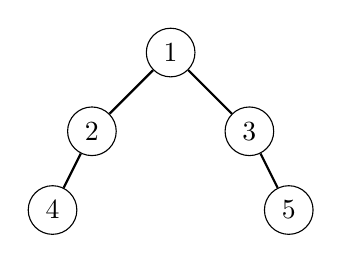
\begin{tikzpicture}[scale=1]
			\node[circle,draw] (1) at (0,1.5) {1};
			\node[circle,draw] (2) at (-1,0.5) {2};
			\node[circle,draw] (3) at (1,0.5) {3};
			\node[circle,draw] (4) at (-1.5,-0.5) {4};
			\node[circle,draw] (5) at (1.5,-0.5) {5};

			\draw[thick] (1) -- (2);
			\draw[thick] (1) -- (3);
			\draw[thick] (2) -- (4);
			\draw[thick] (3) -- (5);
		\end{tikzpicture}
	\end{center}

	\vspace{0.2cm}

	\begin{itemize}
		\item No cycles exist
		\item Graph is already a forest
	\end{itemize}

	\begin{alertblock}{Result}
		FVS = $\emptyset$
	\end{alertblock}

\end{frame}



% --------------------------------------------
\begin{frame}{Visual Example: Simple Cycle}

	\begin{center}
		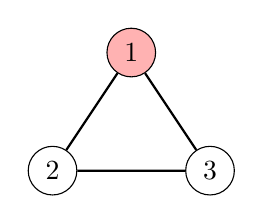
\begin{tikzpicture}[scale=1]
			\node[circle,draw,fill=red!30] (1) at (0,1.5) {1};
			\node[circle,draw] (2) at (-1,0) {2};
			\node[circle,draw] (3) at (1,0) {3};
			\draw[thick] (1) -- (2) -- (3) -- (1);
		\end{tikzpicture}
	\end{center}

	\vspace{0.2cm}

	\begin{itemize}
		\item This graph contains a cycle (triangle)
		\item Removing vertex 1 breaks the cycle
	\end{itemize}

	\begin{alertblock}{Result}
		FVS = $\{1\}$, size = 1
	\end{alertblock}

\end{frame}

% --------------------------------------------
\begin{frame}{Visual Example: Multiple Cycles}

	\begin{center}
		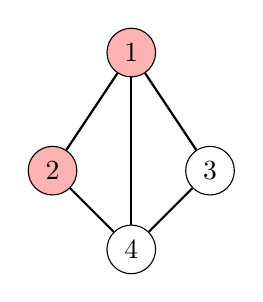
\begin{tikzpicture}[scale=1]
			\node[circle,draw,fill=red!30] (1) at (0,1.5) {1};
			\node[circle,draw,fill=red!30] (2) at (-1,0) {2};
			\node[circle,draw] (3) at (1,0) {3};
			\node[circle,draw] (4) at (0,-1) {4};

			\draw[thick] (1) -- (2) -- (4) -- (3) -- (1);
			\draw[thick] (1) -- (4);
		\end{tikzpicture}
	\end{center}

	\vspace{0.2cm}

	\begin{itemize}
		\item Multiple overlapping cycles exist
		\item Need to remove more vertices
	\end{itemize}

	\begin{alertblock}{Result}
		FVS = $\{1,2\}$
	\end{alertblock}

\end{frame}



% --------------------------------------------
% --------------------------------------------
\begin{frame}{Visual Example: Complex Graph $\rightarrow$ Forest}

	\begin{center}
		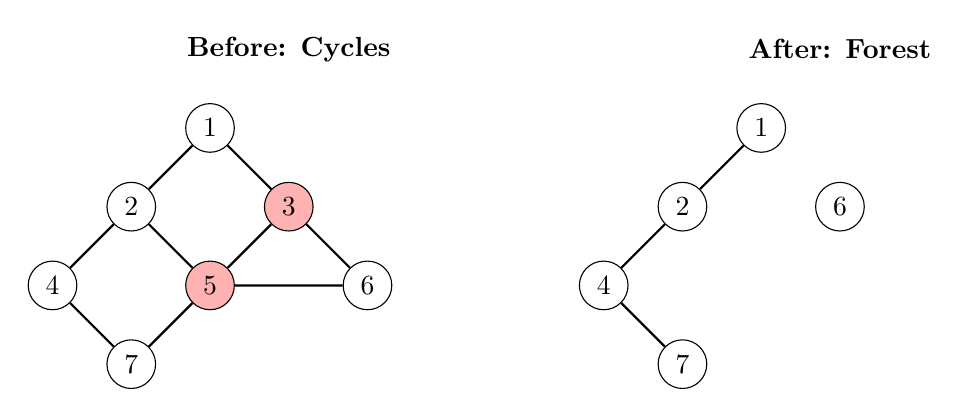
\begin{tikzpicture}[scale=1]
			% ---------------- Before (Left) ----------------
			\node at (-4,3) {\textbf{Before: Cycles}};

			% Nodes
			\node[circle,draw] (B1) at (-5,2) {1};
			\node[circle,draw] (B2) at (-6,1) {2};
			\node[circle,draw,fill=red!30] (B3) at (-4,1) {3};
			\node[circle,draw] (B4) at (-7,0) {4};
			\node[circle,draw,fill=red!30] (B5) at (-5,0) {5};
			\node[circle,draw] (B6) at (-3,0) {6};
			\node[circle,draw] (B7) at (-6,-1) {7};

			% Edges
			\draw[thick] (B1) -- (B2) -- (B4) -- (B7);
			\draw[thick] (B2) -- (B5) -- (B6);
			\draw[thick] (B3) -- (B5);
			\draw[thick] (B1) -- (B3) -- (B6);
			\draw[thick] (B5) -- (B7);

			% ---------------- After (Right) ----------------
			\node at (3,3) {\textbf{After: Forest}};

			% Nodes (removed 3 and 5)
			\node[circle,draw] (A1) at (2,2) {1};
			\node[circle,draw] (A2) at (1,1) {2};
			\node[circle,draw] (A4) at (0,0) {4};
			\node[circle,draw] (A6) at (3,1) {6};
			\node[circle,draw] (A7) at (1,-1) {7};

			% Edges (remaining)
			\draw[thick] (A1) -- (A2) -- (A4) -- (A7);
		\end{tikzpicture}
	\end{center}

	\vspace{0.2cm}

	\begin{itemize}
		\item \textbf{Before:} Multiple cycles exist, highlighted red vertices (3,5) are part of FVS.
		\item \textbf{After:} Removing FVS nodes breaks all cycles $\rightarrow$ Graph becomes a acyclic.
	\end{itemize}

	\begin{alertblock}{Final Verdict}
		FVS = $\{3,5\}$ $\rightarrow$ A set of vertices to remove all cycles.
	\end{alertblock}

\end{frame}






\begin{frame}{Visual Example: Complex Graph $\rightarrow$ Minimal FVS $\rightarrow$ Forest}

	\begin{columns}[T,onlytextwidth]
		% ----------------------------
		% Original Graph
		\column{0.48\textwidth}
		\begin{block}{Original Graph with Cycles}
			\begin{center}
				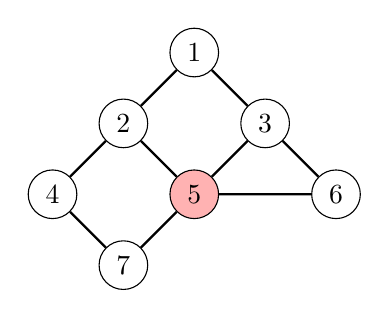
\begin{tikzpicture}[scale=0.9]
					% Nodes
					\node[circle,draw] (1) at (0,2) {1};
					\node[circle,draw] (2) at (-1,1) {2};
					\node[circle,draw] (3) at (1,1) {3};
					\node[circle,draw] (4) at (-2,0) {4};
					\node[circle,draw,fill=red!30] (5) at (0,0) {5};
					\node[circle,draw] (6) at (2,0) {6};
					\node[circle,draw] (7) at (-1,-1) {7};

					% Edges
					\draw[thick] (1) -- (2) -- (4) -- (7);
					\draw[thick] (2) -- (5) -- (6);
					\draw[thick] (3) -- (5);
					\draw[thick] (1) -- (3) -- (6);
					\draw[thick] (5) -- (7);
				\end{tikzpicture}
			\end{center}
		\end{block}

		% ----------------------------
		% Forest After Removing Minimal FVS
		\column{0.48\textwidth}
		\begin{block}{Resulting Forest (Remove 5)}
			\begin{center}
				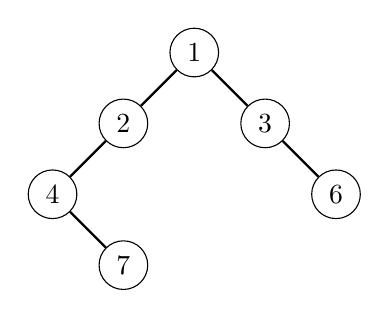
\begin{tikzpicture}[scale=0.9]
					% Nodes (excluding 5)
					\node[circle,draw] (1) at (0,2) {1};
					\node[circle,draw] (2) at (-1,1) {2};
					\node[circle,draw] (3) at (1,1) {3};
					\node[circle,draw] (4) at (-2,0) {4};
					\node[circle,draw] (6) at (2,0) {6};
					\node[circle,draw] (7) at (-1,-1) {7};

					% Edges (only remaining)
					\draw[thick] (1) -- (2) -- (4) -- (7);
					\draw[thick] (1) -- (3);
					\draw[thick] (3) -- (6);
				\end{tikzpicture}
			\end{center}
		\end{block}

	\end{columns}

	\vspace{0.2cm}

	\begin{itemize}
		\item Minimal Feedback Vertex Set: $\{5\}$
		\item Removing vertex 5 breaks all cycles $\rightarrow$ graph becomes a forest
	\end{itemize}

	\begin{alertblock}{Key Insight}
		Even if multiple vertices can break cycles, the \textbf{minimal FVS} is the set with the smallest size.
	\end{alertblock}

\end{frame}











% --------------------------------------------
\begin{frame}{Real-World Motivation}

	\begin{itemize}
		\item \textbf{Deadlocks in Operating Systems:} Cycles in resource allocation graph $\rightarrow$ remove critical process
		\item \textbf{Dependency Resolution:} Packages/modules with circular dependencies $\rightarrow$ remove one to break cycle
		\item \textbf{Circuit Design / Feedback Loops:} Loops in circuits $\rightarrow$ remove components to stabilize
		      % \item \textbf{Social Networks:} Removing influential nodes can break information loops
	\end{itemize}

	\vspace{0.3cm}

	\begin{alertblock}{Insight}
		FVS is a tool to identify minimal critical nodes whose removal resolves all cycles.
	\end{alertblock}

\end{frame}

% --------------------------------------------
\begin{frame}{Key Observations}

	\begin{itemize}
		\item Every cycle must contain at least one removed vertex
		\item Removing fewer vertices is always better
		\item Problem becomes harder as graph becomes denser
	\end{itemize}

	\vspace{0.4cm}

	\begin{block}{Core Insight}
		FVS is about selecting a minimum set of vertices that "hit" all cycles.
	\end{block}

\end{frame}

% % --------------------------------------------
% \begin{frame}{Summary of Intuition}

% \begin{itemize}
%   \item Cycles = structures we want to eliminate
%   \item Removing vertices breaks cycles
%   \item Goal: achieve an acyclic graph (forest)
%   \item Minimize number of removed vertices
% \end{itemize}

% \vspace{0.4cm}

% \begin{alertblock}{Takeaway}
% Feedback Vertex Set = Minimum set of vertices whose removal destroys all cycles.
% \end{alertblock}

% \end{frame}







% ============================================
% PART 2: COMPLEXITY & NP-COMPLETENESS
% ============================================

\section{Complexity and NP-Completeness}

% --------------------------------------------
\begin{frame}{Complexity Overview}

	\begin{block}{Goal of This Section}
		\begin{itemize}
			\item Analyze the \textbf{computational complexity} of FVS
			\item Understand decision vs optimization versions
			\item Prove NP-Completeness using reductions
		\end{itemize}
	\end{block}

\end{frame}

% --------------------------------------------
\begin{frame}{Decision vs Optimization}

	\begin{block}{Decision Version}
		Given $G, k$: Does there exist an FVS of size $\leq k$?
	\end{block}

	\begin{alertblock}{Fact}
		Decision version is \textbf{NP-Complete}
	\end{alertblock}

	\vspace{0.3cm}

	\begin{block}{Optimization Version}
		Find the minimum-size FVS
	\end{block}

	\begin{alertblock}{Fact}
		Optimization version is \textbf{NP-Hard}
	\end{alertblock}

\end{frame}

% --------------------------------------------
\begin{frame}{Main Claim}

	\begin{alertblock}{Theorem}
		The decision version of Feedback Vertex Set is \textbf{NP-Complete}.
	\end{alertblock}

	\vspace{0.3cm}

	\begin{block}{Proof Strategy}
		\begin{enumerate}
			\item Show FVS $\in$ NP
			\item Reduce Vertex Cover $\leq_p$ FVS
		\end{enumerate}
	\end{block}

\end{frame}

% --------------------------------------------
\begin{frame}{Step 1: FVS is in NP}

	\begin{block}{Key Idea (NP Definition)}
		A problem is in NP if a solution can be \textbf{verified in polynomial time}.
	\end{block}

	\vspace{0.3cm}

	\begin{itemize}
		\item Given a set $S$
		\item Remove $S$ from graph
		\item Check if graph has cycles (DFS)
	\end{itemize}

	\vspace{0.3cm}

	\begin{block}{Time Complexity}
		$O(V + E)$
	\end{block}

	\vspace{0.3cm}

	\begin{alertblock}{Conclusion}
		FVS $\in$ NP (verification is polynomial)
	\end{alertblock}

\end{frame}

% --------------------------------------------
\begin{frame}{Step 2: Reduction (VC $\rightarrow$ FVS)}

	\begin{block}{Known Fact}
		Vertex Cover is NP-Complete
	\end{block}

	\vspace{0.3cm}

	\begin{block}{Goal}
		Transform VC instance into FVS instance
	\end{block}

	\vspace{0.3cm}

	\begin{itemize}
		\item Each edge becomes a cycle
		\item FVS must break all cycles
	\end{itemize}

\end{frame}

% ----------------------------------
\begin{frame}{Step 2: Reduction (VC $\rightarrow$ FVS)}
	\begin{block}{Vertex Cover (VC) Problem}
		Find smallest $S \subseteq V$ such that every edge has at least one endpoint in $S$.
	\end{block}

	\vspace{0.3cm}

	\textbf{Construction:} Given VC instance $(G,k)$
	\begin{enumerate}
		\item For each edge $e = (u,v) \in E(G)$:
		      \begin{itemize}
			      \item Add new vertex $w_e$
			      \item Form triangle: edges $(u,v)$, $(u,w_e)$, $(v,w_e)$
		      \end{itemize}
		\item Keep same parameter $k' = k$
	\end{enumerate}

	\vspace{0.3cm}

	\begin{theorem}
		$G$ has VC of size $\leq k$ $\Leftrightarrow$ $G'$ has \fvs\ of size $\leq k$
	\end{theorem}

	\textbf{Time:} $O(|E|)$ (polynomial)
\end{frame}


% --------------------------------------------
\begin{frame}{Reduction Construction (Graph)}

	\begin{center}
		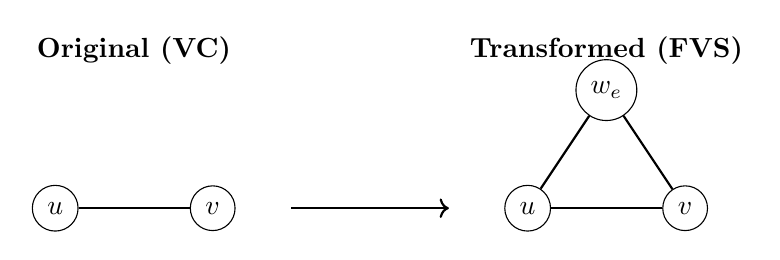
\begin{tikzpicture}[scale=1]

			\node at (-3,2) {\textbf{Original (VC)}};

			\node[circle,draw] (u) at (-4,0) {$u$};
			\node[circle,draw] (v) at (-2,0) {$v$};

			\draw[thick] (u) -- (v);

			\draw[->,thick] (-1,0) -- (1,0);

			\node at (3,2) {\textbf{Transformed (FVS)}};

			\node[circle,draw] (u2) at (2,0) {$u$};
			\node[circle,draw] (v2) at (4,0) {$v$};
			\node[circle,draw] (w) at (3,1.5) {$w_e$};

			\draw[thick] (u2) -- (v2);
			\draw[thick] (u2) -- (w);
			\draw[thick] (v2) -- (w);

		\end{tikzpicture}
	\end{center}

	\vspace{0.3cm}

	\begin{itemize}
		\item Each edge becomes a triangle
		\item Triangle = cycle $\rightarrow$ must be broken
	\end{itemize}

\end{frame}

% --------------------------------------------
% ✅ ADDED YOUR BIG VISUAL (KEEPING IT)
% --------------------------------------------
\begin{frame}{VC $\rightarrow$ FVS: Full Graph Illustration}

	\begin{columns}[T]
		\column{0.45\textwidth}

		\textbf{Original Graph}
		\begin{center}
			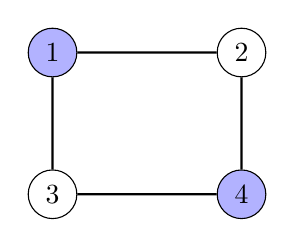
\begin{tikzpicture}[scale=1.2]
				\node[circle,draw,fill=blue!30] (1) at (0,1.5) {1};
				\node[circle,draw] (2) at (2,1.5) {2};
				\node[circle,draw] (3) at (0,0) {3};
				\node[circle,draw,fill=blue!30] (4) at (2,0) {4};

				\draw[thick] (1)--(2)--(4)--(3)--(1);
			\end{tikzpicture}
		\end{center}

		\small VC = $\{1,4\}$

		\column{0.55\textwidth}

		\textbf{Transformed Graph}
		\begin{center}
			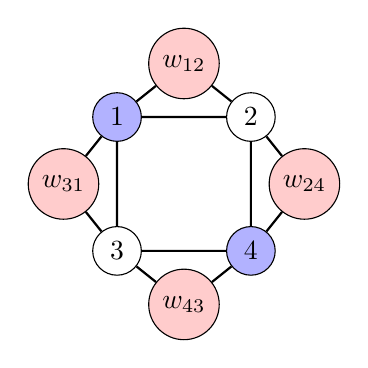
\begin{tikzpicture}[scale=0.85]
				\node[circle,draw,fill=blue!30] (1) at (0,2) {1};
				\node[circle,draw] (2) at (2,2) {2};
				\node[circle,draw] (3) at (0,0) {3};
				\node[circle,draw,fill=blue!30] (4) at (2,0) {4};

				\node[circle,draw,fill=red!20] (w12) at (1,2.8) {$w_{12}$};
				\node[circle,draw,fill=red!20] (w24) at (2.8,1) {$w_{24}$};
				\node[circle,draw,fill=red!20] (w43) at (1,-0.8) {$w_{43}$};
				\node[circle,draw,fill=red!20] (w31) at (-0.8,1) {$w_{31}$};

				\draw[thick] (1)--(2)--(w12)--(1);
				\draw[thick] (2)--(4)--(w24)--(2);
				\draw[thick] (4)--(3)--(w43)--(4);
				\draw[thick] (3)--(1)--(w31)--(3);
			\end{tikzpicture}
		\end{center}

		\small Each triangle = one edge

	\end{columns}

	\vspace{0.3cm}

	\begin{block}{Key Insight}
		Breaking all triangles = covering all edges
	\end{block}

\end{frame}

% --------------------------------------------
\begin{frame}{Correctness of Reduction}

	\begin{block}{Claim}
		$G$ has a VC of size $\leq k$
		$\Longleftrightarrow$
		$G'$ has an FVS of size $\leq k$
	\end{block}

	\textbf{Forward:}
	\begin{itemize}
		\item VC selects endpoints $\rightarrow$ every triangle broken
	\end{itemize}

	\textbf{Backward:}
	\begin{itemize}
		\item FVS must hit each triangle
		\item Implies every edge is covered
	\end{itemize}

\end{frame}

% --------------------------------------------
\begin{frame}{Polynomial Time Reduction}

	\begin{itemize}
		\item Add one vertex per edge
		\item Linear size increase
	\end{itemize}

	\begin{alertblock}{Conclusion}
		Reduction runs in polynomial time
	\end{alertblock}

\end{frame}




\begin{frame}{Reverse Reduction (FVS $\rightarrow$ VC)}
	\begin{block}{Reverse Direction}
		Shows Vertex Cover and \fvs\ are polynomially equivalent
	\end{block}

	\vspace{0.3cm}

	\textbf{Construction:} Given \fvs\ instance $(G,k)$
	\begin{enumerate}
		\item Replace each vertex $v \in V$ with triangle $\{v_1, v_2, v_3\}$
		\item For each edge $(u,v) \in E$, connect triangles with cross edges
		\item Set $k' = 2|V| + k$
	\end{enumerate}

	\vspace{0.3cm}

	\begin{theorem}
		$G$ has \fvs\ of size $\leq k$ $\Leftrightarrow$ $G'$ has VC of size $\leq 2|V| + k$
	\end{theorem}

	\textbf{Key Insight:}
	\begin{itemize}
		\item Each triangle needs $\geq 2$ vertices in VC
		\item Triangles with 3 vertices in VC, $\leftrightarrow$ vertices in \fvs
	\end{itemize}
\end{frame}



\begin{frame}{\fvs $\rightarrow$ VC: Visual Example}

	\begin{block}{Idea}
		Show structural similarity between problems
	\end{block}

	\vspace{0.3cm}

	\begin{columns}
		\column{0.4\textwidth}

		\textbf{Original Graph}
		\begin{center}
			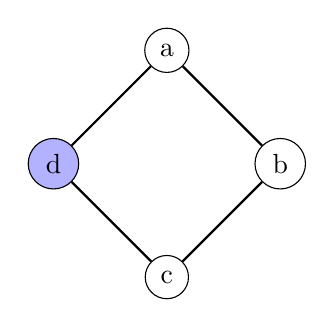
\begin{tikzpicture}[scale=1.2]
				\node[circle,draw] (a) at (90:1.2) {a};
				\node[circle,draw] (b) at (0:1.2) {b};
				\node[circle,draw] (c) at (270:1.2) {c};
				\node[circle,draw,fill=blue!30] (d) at (180:1.2) {d};

				\draw[thick] (a)--(b)--(c)--(d)--(a);
			\end{tikzpicture}
		\end{center}

		\small FVS = $\{d\}$

		\column{0.6\textwidth}

		\textbf{Construction}
		\begin{itemize}
			\item Each vertex $\rightarrow$ triangle
			\item Selecting all 3, $\leftrightarrow$ remove vertex
			\item Selecting 2, $\leftrightarrow$ keep vertex
		\end{itemize}

	\end{columns}

	\vspace{0.3cm}

	% \begin{alertblock}{Insight}
	% FVS and Vertex Cover are structurally related
	% \end{alertblock}

\end{frame}


\begin{frame}{\fvs $\rightarrow$ VC: Visual Example}
	\begin{columns}[T]
		\column{0.4\textwidth}
		\textbf{Original Graph $G$:}
		\begin{center}
			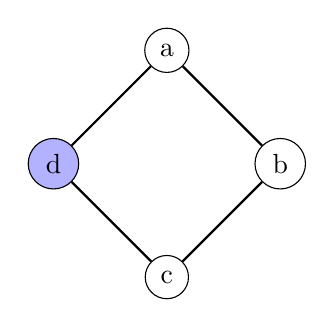
\begin{tikzpicture}[scale=1.2]
				\node[circle,draw] (a) at (90:1.2) {a};
				\node[circle,draw] (b) at (0:1.2) {b};
				\node[circle,draw] (c) at (270:1.2) {c};
				\node[circle,draw,fill=blue!30] (d) at (180:1.2) {d};
				\draw[thick] (a) -- (b) -- (c) -- (d) -- (a);
			\end{tikzpicture}
		\end{center}
		\small
		\fvs: $\{d\}$ (size=1)\\
		Removing $d$ breaks the 4-cycle

		\column{0.6\textwidth}
		\textbf{Transformed Graph $G'$:}
		\begin{center}
			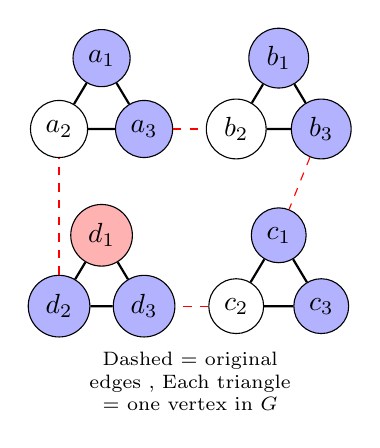
\begin{tikzpicture}[scale=0.9]
				% Triangles spaced out
				\node[circle,draw,fill=blue!30] (a1) at (0,2.5) {$a_1$};
				\node[circle,draw] (a2) at (-0.6,1.5) {$a_2$};
				\node[circle,draw,fill=blue!30] (a3) at (0.6,1.5) {$a_3$};
				\draw[thick] (a1) -- (a2) -- (a3) -- (a1);

				\node[circle,draw,fill=blue!30] (b1) at (2.5,2.5) {$b_1$};
				\node[circle,draw] (b2) at (1.9,1.5) {$b_2$};
				\node[circle,draw,fill=blue!30] (b3) at (3.1,1.5) {$b_3$};
				\draw[thick] (b1) -- (b2) -- (b3) -- (b1);

				\node[circle,draw,fill=red!30] (d1) at (0,0) {$d_1$};
				\node[circle,draw,fill=blue!30] (d2) at (-0.6,-1) {$d_2$};
				\node[circle,draw,fill=blue!30] (d3) at (0.6,-1) {$d_3$};
				\draw[thick] (d1) -- (d2) -- (d3) -- (d1);

				\node[circle,draw,fill=blue!30] (c1) at (2.5,0) {$c_1$};
				\node[circle,draw] (c2) at (1.9,-1) {$c_2$};
				\node[circle,draw,fill=blue!30] (c3) at (3.1,-1) {$c_3$};
				\draw[thick] (c1) -- (c2) -- (c3) -- (c1);

				% Representative cross edges (just show pattern)
				\draw[dashed,red] (a3) -- (b2);
				\draw[dashed,red] (b3) -- (c1);
				\draw[dashed,red] (c2) -- (d3);
				\draw[dashed,red] (d2) -- (a2);

				\node[text width=3cm,align=center,font=\scriptsize] at (1.25,-2) {\\Dashed = original edges , Each triangle = one vertex in $G$};
			\end{tikzpicture}
		\end{center}
	\end{columns}

	\vspace{0.3cm}
	\begin{minipage}{\textwidth}
		\small
		\textbf{Vertex Cover in $G'$:(with d1) is a FVS in  $G'$}
		% \begin{itemize}
		%   \item Choose \textbf{all 3} from triangle $d$ (blue) $\rightarrow$ vertex $d$ in \fvs
		%   \item Choose \textbf{2 from each} of triangles $a,b,c$ $\rightarrow$ vertices not in \fvs
		%   \item Total size = $3 + 2+2+2 = 9$
		%   \item Formula: $2|V| + k = 2\times4 + 1 = 9$ ✓
		% \end{itemize}
	\end{minipage}
\end{frame}
% --------------------------------------------
% ✅ YOUR SECOND VISUAL KEPT
% --------------------------------------------


% --------------------------------------------
\begin{frame}{Final Conclusion}

	\begin{block}{We Have Proven}
		\begin{itemize}
			\item FVS $\in$ NP
			\item Vertex Cover $\leq_p$ FVS
			\item VC is NP-Complete
		\end{itemize}
	\end{block}

	\vspace{0.4cm}

	\begin{alertblock}{Final Verdict}
		\textbf{Feedback Vertex Set (Decision) is NP-Complete}
	\end{alertblock}

	\vspace{0.3cm}

	\begin{block}{Implication}
		\begin{itemize}
			\item Optimization version is NP-Hard
			\item No known polynomial-time exact algorithm
		\end{itemize}
	\end{block}

\end{frame}




% ============================================
% PART 2: EXISTING ALGORITHMS (COMPLETE)
% ============================================

\section{Existing Algorithms Survey}


% --------------------------------------------
\begin{frame}{Approaches to Solving FVS: Algorithmic Survey}


\begin{block}{Major Categories of Solution Approaches}
\begin{itemize}
    \item Exact Exponential Algorithms
    \item Approximation Algorithms
    \item Randomized Algorithms
    \item Heuristic Methods
    \item Metaheuristic Techniques
\end{itemize}
\end{block}

\vspace{0.3cm}

\begin{alertblock}{Objective}
Provide a comprehensive overview of existing algorithms,
their complexity, and practical trade-offs.
\end{alertblock}

\end{frame}

% =====================================================
% EXACT EXPONENTIAL
% =====================================================

\begin{frame}{Exact Exponential Algorithms}

\begin{block}{Idea}
Guarantee optimal solutions using exhaustive search or parameterized techniques.
\end{block}

\vspace{0.2cm}

\begin{exampleblock}{Use Cases}
\begin{itemize}
\item When exact solution is required
\item Small graphs or small parameter $k$
\end{itemize}
\end{exampleblock}

\vspace{0.2cm}

\begin{alertblock}{Algorithms}

\begin{columns}[T] % T = top alignment
\column{0.5\textwidth}
\begin{itemize}
\item Naive Brute Force
\item DP on Subsets
\item Iterative Compression
\end{itemize}

\column{0.5\textwidth}
\begin{itemize}
\item Bounded Search Tree
\item Current Best FPT
\item Inclusion-Exclusion DP
\end{itemize}

\end{columns}

\end{alertblock}

\end{frame}



% --------------------------------------------
\begin{frame}{Naive Brute Force}

\begin{block}{Algorithm Steps}
\begin{itemize}
\item Generate all subsets of vertices
\item For each subset, remove vertices from graph
\item Check if resulting graph is acyclic
\item Return smallest valid subset
\end{itemize}
\end{block}

\vspace{0.2cm}

\begin{exampleblock}{Complexity}
$O(2^n \cdot n^3)$
\end{exampleblock}

\vspace{0.2cm}

\begin{alertblock}{Reference}
\href{https://perso.limos.fr/~palafour/PAPERS/PDF/Garey-Johnson79.pdf}{Garey \& Johnson (1979)}
\end{alertblock}

\end{frame}
% --------------------------------------------
\begin{frame}{DP on Subsets}

\begin{block}{Algorithm Steps}
\begin{itemize}
\item Enumerate subsets of vertices
\item Store intermediate results using DP
\item Avoid recomputation of overlapping subsets
\item Select minimum valid FVS
\end{itemize}
\end{block}

\begin{exampleblock}{Complexity}
$O(2^n \cdot n^2)$
\end{exampleblock}

\begin{alertblock}{Reference}
\href{https://mimuw.edu.pl/~malcin/book/parameterized-algorithms.pdf}{Cygan et al., Parameterized Algorithms (2015)}
\end{alertblock}

\end{frame}

% --------------------------------------------
\begin{frame}{Iterative Compression}

\begin{block}{Algorithm Steps}
\begin{itemize}
\item Start with small subgraph solution
\item Add vertices incrementally
\item Maintain solution of size $k+1$
\item Compress solution to size $k$
\end{itemize}
\end{block}

\begin{exampleblock}{Complexity}
$O(5^k \cdot kn^2)$
\end{exampleblock}

\begin{alertblock}{Reference}
\href{https://dehne73176131.wordpress.com/wp-content/uploads/2017/12/1-45.pdf}{Dehne et al., Theory of Computing Systems (2007)}
\end{alertblock}

\end{frame}

% --------------------------------------------
\begin{frame}{Bounded Search Tree}

\begin{block}{Algorithm Steps}
\begin{itemize}
\item Detect a cycle in the graph
\item Select a vertex from the cycle
\item Branch by removing each possible vertex
\item Recurse until graph becomes acyclic or $k$ exhausted
\end{itemize}
\end{block}

\begin{exampleblock}{Complexity}
$O(4^k \cdot n^2)$
\end{exampleblock}

\begin{alertblock}{Reference}
  % 1
\href{https://doi.org/10.1007/s00453-008-9215-6}{Chen et al. (2008)}
\end{alertblock}

\end{frame}

% --------------------------------------------
\begin{frame}{Current Best FPT}

\begin{block}{Algorithm Steps}
\begin{itemize}
\item Apply reduction and kernelization rules
\item Use advanced branching strategies
\item Reduce problem size iteratively
\item Solve using optimized search tree
\end{itemize}
\end{block}

\begin{exampleblock}{Complexity}
$O(3.619^k \cdot n^4)$
\end{exampleblock}

\begin{alertblock}{Reference}
\href{https://doi.org/10.1016/j.jcss.2008.05.002}{Chen et al., Journal of Computer and System Sciences (2008)}
\end{alertblock}

\end{frame}

% --------------------------------------------
\begin{frame}{Inclusion-Exclusion DP}

\begin{block}{Algorithm Steps}
\begin{itemize}
\item Enumerate subsets using inclusion-exclusion principle
\item Count valid configurations using DP
\item Avoid overcounting via inclusion-exclusion
\item Select subset forming valid FVS
\end{itemize}
\end{block}

\begin{exampleblock}{Complexity}
$O(2^n \cdot n)$
\end{exampleblock}

\begin{alertblock}{Reference}
\href{https://epubs.siam.org/doi/10.1137/1.9781611973099.139}{Björklund et al. (2010)}
\end{alertblock}

\end{frame}

% =====================================================
% APPROXIMATION
% =====================================================

\begin{frame}{Approximation Algorithms}

\begin{block}{Idea}
Provide near-optimal solutions with provable approximation guarantees.
\end{block}

\vspace{0.2cm}

\begin{exampleblock}{Use Cases}
\begin{itemize}
\item When exact solution is computationally infeasible
\item Large graphs where guarantees are required
\end{itemize}
\end{exampleblock}

\vspace{0.2cm}

\begin{alertblock}{Algorithms}

\begin{columns}[T]
\column{0.5\textwidth}
\begin{itemize}
\item 2-Approximation (VC-based)
\item Log-Approximation
\end{itemize}

\column{0.5\textwidth}
\begin{itemize}
\item LP Rounding
\item Primal-Dual
\end{itemize}

\end{columns}

\end{alertblock}

\end{frame}

% --------------------------------------------
\begin{frame}{2-Approximation (VC-based)}

\begin{block}{Algorithm Steps}
\begin{itemize}
\item Find a cycle in the graph
\item Select an edge from the cycle
\item Remove both endpoints of the edge
\item Repeat until graph becomes acyclic
\end{itemize}
\end{block}

\begin{exampleblock}{Approximation Guarantee}
$\leq 2 \times OPT$
\end{exampleblock}

\begin{alertblock}{Reference}
\href{https://csaws.cs.technion.ac.il/~reuven/SAVE/OTHERS/vfs_bafna.pdf}{Bafna et al. (1999)}
\end{alertblock}

\end{frame}
% --------------------------------------------
\begin{frame}{Log-Approximation}

\begin{block}{Algorithm Steps}
\begin{itemize}
\item Convert problem into hitting set formulation
\item Identify sets corresponding to cycles
\item Apply greedy/log approximation algorithm
\item Select vertices covering all cycles
\end{itemize}
\end{block}

\begin{exampleblock}{Approximation Guarantee}
$O(\log n)$
\end{exampleblock}

\begin{alertblock}{Reference}
\href{https://doi.org/10.1137/S0097539796303400}{Bar-Yehuda (Approximation for FVS)}
\end{alertblock}

\end{frame}

% --------------------------------------------
\begin{frame}{LP Rounding}

\begin{block}{Algorithm Steps}
\begin{itemize}
\item Formulate FVS as integer linear program
\item Relax constraints to linear program
\item Solve LP to obtain fractional solution
\item Round values to obtain integer solution
\end{itemize}
\end{block}

\begin{exampleblock}{Complexity}
$O(n^{3.5})$
\end{exampleblock}

\begin{alertblock}{Reference}
\href{https://doi.org/10.1145/227234.227238}{Bar-Yehuda \& Even (1985)}
\end{alertblock}

\end{frame}

% --------------------------------------------
\begin{frame}{Primal-Dual}

\begin{block}{Algorithm Steps}
\begin{itemize}
\item Initialize primal and dual solutions
\item Increase dual variables iteratively
\item Select vertices when constraints become tight
\item Construct feasible FVS solution
\end{itemize}
\end{block}

\begin{exampleblock}{Complexity}
$O(n^2)$
\end{exampleblock}

\begin{alertblock}{Reference}
  \href{https://dl.acm.org/doi/pdf/10.1145/227683.227684}{Goemans \& Williamson (1995)}
\end{alertblock}

\end{frame}

% =====================================================
% RANDOMIZED
% =====================================================

\begin{frame}{Randomized Algorithms}

\begin{block}{Idea}
Use randomness to achieve good expected performance and scalability.
\end{block}

\vspace{0.2cm}

\begin{exampleblock}{Use Cases}
\begin{itemize}
\item When probabilistic guarantees are acceptable
\item Large-scale graphs with time constraints
\end{itemize}
\end{exampleblock}

\vspace{0.2cm}

\begin{alertblock}{Algorithms}

\begin{columns}[T]
\column{0.5\textwidth}
\begin{itemize}
\item Random Sampling
\item Randomized Rounding
\end{itemize}

\column{0.5\textwidth}
\begin{itemize}
\item Color Coding
\end{itemize}

\end{columns}

\end{alertblock}

\end{frame}

% --------------------------------------------
\begin{frame}{Random Sampling}

\begin{block}{Algorithm Steps}
\begin{itemize}
\item Randomly select a vertex from graph
\item Check if it belongs to a cycle
\item Add it to solution if needed
\item Repeat multiple times and choose best result
\end{itemize}
\end{block}

\begin{exampleblock}{Performance}
Expected $O(\log n)$ approximation
\end{exampleblock}

\begin{alertblock}{Reference}
\href{https://doi.org/10.1017/CBO9780511814075}{Motwani \& Raghavan, Randomized Algorithms}
\end{alertblock}

\end{frame}

% --------------------------------------------
\begin{frame}{Randomized Rounding}

\begin{block}{Algorithm Steps}
\begin{itemize}
\item Solve LP relaxation
\item Interpret fractional values as probabilities
\item Randomly select vertices based on probability
\item Repeat and select best solution
\end{itemize}
\end{block}

\begin{exampleblock}{Guarantee}
Expected 2-approximation
\end{exampleblock}

\begin{alertblock}{Reference}
\href{https://doi.org/10.1007/978-3-662-04565-7}{Vazirani (2001)}
\end{alertblock}

\end{frame}

% --------------------------------------------
\begin{frame}{Color Coding}

\begin{block}{Algorithm Steps}
\begin{itemize}
\item Assign random colors to vertices
\item Identify colorful structures
\item Use dynamic programming to detect solutions
\item Repeat to improve probability
\end{itemize}
\end{block}

\begin{exampleblock}{Complexity}
$O(2^{O(k)} \cdot n)$
\end{exampleblock}

\begin{alertblock}{Reference}
\href{https://doi.org/10.1145/210332.210337}{Alon, Yuster, Zwick (1995)}
\end{alertblock}

\end{frame}

% =====================================================
% HEURISTIC
% =====================================================

\begin{frame}{Heuristic Algorithms}

\begin{block}{Idea}
Provide fast and practical solutions without theoretical guarantees.
\end{block}

\vspace{0.2cm}

\begin{exampleblock}{Use Cases}
\begin{itemize}
\item Real-world applications requiring fast solutions
\item Very large graphs where exact methods fail
\end{itemize}
\end{exampleblock}

\vspace{0.2cm}

\begin{alertblock}{Algorithms}

\begin{columns}[T]
\column{0.5\textwidth}
\begin{itemize}
\item Greedy Vertex Selection
\item Cycle-Based Greedy
\item Maximum Degree Heuristic
\end{itemize}

\column{0.5\textwidth}
\begin{itemize}
\item Core-Periphery Decomposition
\item Reduction Rules + Greedy
\end{itemize}

\end{columns}

\end{alertblock}

\end{frame}

% --------------------------------------------
\begin{frame}{Greedy Vertex Selection}

\begin{block}{Algorithm Steps}
\begin{itemize}
\item Compute degrees of all vertices
\item Select highest-degree vertex
\item Remove it from graph
\item Repeat until no cycles remain
\end{itemize}
\end{block}

\begin{exampleblock}{Complexity}
$O(n^2 \log n)$
\end{exampleblock}

\begin{alertblock}{Reference}
\href{https://doi.org/10.1016/j.tcs.2004.12.001}{Festa et al., Theoretical Computer Science (2004)}
\end{alertblock}

\end{frame}

% --------------------------------------------
\begin{frame}{Cycle-Based Greedy}

\begin{block}{Algorithm Steps}
\begin{itemize}
\item Detect cycles using DFS/BFS
\item Count vertex participation in cycles
\item Select most frequent vertex
\item Remove and repeat
\end{itemize}
\end{block}

\begin{exampleblock}{Complexity}
$O(n^3)$
\end{exampleblock}

\begin{alertblock}{Reference}
\href{https://doi.org/10.1016/j.ejor.2007.01.060}{Festa et al., European Journal of Operational Research (2008)}
\end{alertblock}

\end{frame}

% --------------------------------------------
\begin{frame}{Maximum Degree Heuristic}

\begin{block}{Algorithm Steps}
\begin{itemize}
\item Compute vertex degrees
\item Apply tie-breaking rules
\item Remove highest scoring vertex
\item Repeat until acyclic
\end{itemize}
\end{block}

\begin{exampleblock}{Complexity}
$O(n^2 \log n)$
\end{exampleblock}

\begin{alertblock}{Reference}
\href{https://doi.org/10.1016/j.dam.2005.05.007}{Fomin et al., Discrete Applied Mathematics (2006)}
\end{alertblock}

\end{frame}

% --------------------------------------------
\begin{frame}{Core-Periphery Decomposition}

\begin{block}{Algorithm Steps}
\begin{itemize}
\item Compute k-core decomposition
\item Identify dense core region
\item Focus removal on core vertices
\item Apply greedy selection
\end{itemize}
\end{block}

\begin{exampleblock}{Complexity}
$O(n + m)$
\end{exampleblock}

\begin{alertblock}{Reference}
  %2
\href{https://doi.org/10.1137/1.9781611972832.4}{Batagelj \& Zaversnik, SIAM (2003)}
\end{alertblock}

\end{frame}

% --------------------------------------------
\begin{frame}{Reduction Rules + Greedy}

\begin{block}{Algorithm Steps}
\begin{itemize}
\item Remove degree $\leq 1$ vertices
\item Contract degree-2 vertices
\item Apply preprocessing rules
\item Run greedy on reduced graph
\end{itemize}
\end{block}

\begin{exampleblock}{Complexity}
$O(n^2)$
\end{exampleblock}

\begin{alertblock}{Reference}
  %3
\href{https://link.springer.com/chapter/10.1007/978-3-642-11269-0_2}{Kernelization: New Upper and Lower Bound Techniques}
\end{alertblock}

\end{frame}

% =====================================================
% METAHEURISTIC
% =====================================================

\begin{frame}{Metaheuristic Algorithms}

\begin{block}{Idea}
Use global optimization techniques to explore large solution spaces.
\end{block}

\vspace{0.2cm}

\begin{exampleblock}{Use Cases}
\begin{itemize}
\item Complex large-scale graphs
\item When near-optimal solutions are acceptable
\end{itemize}
\end{exampleblock}

\vspace{0.2cm}

\begin{alertblock}{Algorithms}

\begin{columns}[T]
\column{0.5\textwidth}
\begin{itemize}
\item Genetic Algorithm
\item Simulated Annealing
\item Ant Colony Optimization
\end{itemize}

\column{0.5\textwidth}
\begin{itemize}
\item Tabu Search
\item Particle Swarm Optimization
\end{itemize}

\end{columns}

\end{alertblock}

\end{frame}

% --------------------------------------------
\begin{frame}{Genetic Algorithm}

\begin{block}{Algorithm Steps}
\begin{itemize}
\item Initialize population randomly
\item Evaluate fitness of solutions
\item Apply crossover and mutation
\item Select best individuals iteratively
\end{itemize}
\end{block}

\begin{exampleblock}{Complexity}
$O(g \cdot p \cdot n^2)$
\end{exampleblock}

\begin{alertblock}{Reference}
\href{https://mitpress.mit.edu/9780262031417/genetic-algorithms-in-search-optimization-and-machine-learning/}{Goldberg (1989)}
\end{alertblock}

\end{frame}

% --------------------------------------------
\begin{frame}{Simulated Annealing}

\begin{block}{Algorithm Steps}
\begin{itemize}
\item Start with initial solution
\item Generate neighboring solution
\item Accept worse solutions probabilistically
\item Gradually decrease temperature
\end{itemize}
\end{block}

\begin{exampleblock}{Complexity}
$O(i \cdot n^2)$
\end{exampleblock}

\begin{alertblock}{Reference}
\href{https://www.science.org/doi/10.1126/science.220.4598.671}{Kirkpatrick et al. (1983)}
\end{alertblock}

\end{frame}

% --------------------------------------------
\begin{frame}{Ant Colony Optimization}

\begin{block}{Algorithm Steps}
\begin{itemize}
\item Initialize pheromone levels
\item Construct solutions probabilistically
\item Update pheromones based on quality
\item Repeat for multiple iterations
\end{itemize}
\end{block}

\begin{exampleblock}{Complexity}
$O(\text{ants} \cdot i \cdot n^2)$
\end{exampleblock}

\begin{alertblock}{Reference}
\href{https://ieeexplore.ieee.org/document/585892}{Dorigo \& Gambardella (1997)}
\end{alertblock}

\end{frame}

% --------------------------------------------
\begin{frame}{Tabu Search}

\begin{block}{Algorithm Steps}
\begin{itemize}
\item Start with initial solution
\item Explore neighborhood solutions
\item Maintain tabu list to avoid repetition
\item Update best solution found
\end{itemize}
\end{block}

\begin{exampleblock}{Complexity}
$O(i \cdot n^2)$
\end{exampleblock}

\begin{alertblock}{Reference}
\href{https://pubsonline.informs.org/doi/pdf/10.1287/ijoc.1.3.190}{Glover (1989)}
\end{alertblock}

\end{frame}

% --------------------------------------------
\begin{frame}{Particle Swarm Optimization}

\begin{block}{Algorithm Steps}
\begin{itemize}
\item Initialize swarm of particles
\item Update velocity and position
\item Share global and local best
\item Iterate until convergence
\end{itemize}
\end{block}

\begin{exampleblock}{Complexity}
$O(\text{particles} \cdot i \cdot n^2)$
\end{exampleblock}

\begin{alertblock}{Reference}
\href{https://ieeexplore.ieee.org/document/488968}{Kennedy \& Eberhart (1995)}
\end{alertblock}

\end{frame}

\section{Our implementations}

\begin{frame}{Algorithm Selection Criteria}
	\begin{columns}[T]
		\column{0.36\textwidth}
		\begin{block}{Essential Criteria}
			\footnotesize
			\textbf{1. Implementability}
			\begin{itemize}
				\item Feasible in 6-week timeframe
				\item Well-documented in literature
				\item Reasonable debugging complexity
			\end{itemize}

			\textbf{2. Research Potential}
			\begin{itemize}
				\item Novel comparisons possible
				\item Room for improvements
				\item Publishable results
			\end{itemize}

			\textbf{3. Complementary Nature}
			\begin{itemize}
				\item Different problem sizes
				\item Different paradigms
				\item Interesting comparisons
			\end{itemize}
		\end{block}

		\column{0.36\textwidth}
		\begin{block}{Additional Criteria}
			\footnotesize
			\textbf{4. Practical Relevance}
			\begin{itemize}
				\item Real-world applications
				\item Industry interest
				\item Addresses practical needs
			\end{itemize}

			\textbf{5. Educational Value}
			\begin{itemize}
				\item Learn important techniques
				\item Transferable skills
				\item Deep algorithmic insights
			\end{itemize}
		\end{block}

		\begin{alertblock}{Goal}
			\footnotesize
			Select algorithms that maximize research impact while ensuring feasibility
		\end{alertblock}
	\end{columns}
\end{frame}

\begin{frame}{Selected Algorithms for Implementation}
	\begin{block}{Three-Algorithm Approach (Maximum Research Impact)}
		We will implement three complementary algorithms covering the entire solution spectrum:
	\end{block}

	\vspace{0.3cm}

	\begin{enumerate}
		\item \textbf{Iterative Compression} (Exact FPT Algorithm)
		      \begin{itemize}
			      \footnotesize
			      \item Guarantees optimal solution for small-medium $k$
			      \item Time: $O(5^k \cdot kn^2)$ --- FPT breakthrough (2004)
			      \item Research: Hybrid approaches, parallelization, adaptive branching
		      \end{itemize}

		      \vspace{0.2cm}

		\item \textbf{Kernelization + Bounded Search Tree} (Enhanced Exact)
		      \begin{itemize}
			      \footnotesize
			      \item Preprocessing with reduction rules + exact search
			      \item Kernel reduction: 50-90\% for many graph types
			      \item Research: New reduction rules, smart branching strategies
		      \end{itemize}

		      \vspace{0.2cm}

		\item \textbf{Memetic Algorithm} (Advanced GA + Local Search)
		      \begin{itemize}
			      \footnotesize
			      \item Handles large instances (n $>$ 1000)
			      \item Combines population evolution with local optimization
			      \item Research: Problem-specific operators, ML integration, hybrid exact-metaheuristic
		      \end{itemize}
	\end{enumerate}
\end{frame}

\begin{frame}{Algorithm 1: Iterative Compression (IC)}
	\begin{columns}[T]
		\column{0.48\textwidth}
		\begin{block}{Core Concept}
			\footnotesize
			Given FVS of size $k+1$, compress it to size $k$ through smart enumeration
		\end{block}

		\textbf{Theoretical Significance:}
		\begin{itemize}
			\footnotesize
			\item Most important FPT technique
			\item Published in STOC/FOCS
			\item Demonstrates advanced understanding
		\end{itemize}

		\vspace{0.2cm}

		\textbf{Implementation:}
		\begin{itemize}
			\footnotesize
			\item Complexity: Medium
			\item Expected range: $k \leq 30$
			\item Validation on small instances
		\end{itemize}

		\column{0.48\textwidth}
		\textbf{Research Directions:}
		\begin{enumerate}
			\footnotesize
			\item \textbf{Hybrid Kernelization + IC}
			      \begin{itemize}
				      \scriptsize
				      \item Apply reduction rules before IC
				      \item Potential 2-5x speedup
			      \end{itemize}

			\item \textbf{Adaptive Branching}
			      \begin{itemize}
				      \scriptsize
				      \item Learn which vertices to branch first
				      \item Use graph structure metrics
			      \end{itemize}

			\item \textbf{Parallelization}
			      \begin{itemize}
				      \scriptsize
				      \item Independent branches in parallel
				      \item Multi-core speedup potential
			      \end{itemize}

			\item \textbf{Improved Compression}
			      \begin{itemize}
				      \scriptsize
				      \item Smart partition enumeration
				      \item Structure-based pruning
			      \end{itemize}
		\end{enumerate}

	\end{columns}
\end{frame}

\begin{frame}{Iterative Compression for FVS}
	\small
	\textbf{Idea:} Build solution incrementally and compress when too large.

	\textbf{Algorithm}
	{\small
		\setlength{\baselineskip}{8pt}
		\begin{algorithmic}[1]
			\State Order vertices $v_1,\dots,v_n$
			\State $F \gets \{v_1\}$
			\For{$i = 2$ to $n$}
			\State $F \gets F \cup \{v_i\}$
			\If{$|F| = k+1$}
			\ForAll{partitions $(F_1,F_2)$ of $F$}
			\State find $Y \subseteq V \setminus F_2$
			\If{$F_1 \cup Y$ is an FVS}
			\State update $F$ and \textbf{break}
			\EndIf
			\EndFor
			\If{no update performed}
			\State \textbf{return NO}
			\EndIf
			\EndIf
			\EndFor
			\State \textbf{return} $F$ \textbf{if} $|F| \le k$
		\end{algorithmic}
	}


	\textbf{Key Insight:} Compress size $k\!+\!1$ to $k$ \\
	\textbf{Time:} $O(5^k \cdot n^2)$
\end{frame}

\begin{frame}{Simulation}
	\textbf{Simulation of FVS (k=2) on 5 vertices}

	% ---------- STEP 1 ----------
	\textbf{Step 1: $F=\{A\}$}
	\begin{center}

		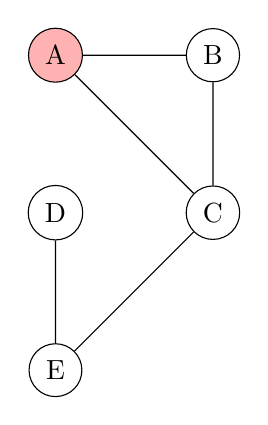
\begin{tikzpicture}[node distance=2cm]
			\node[draw, circle, fill=red!30] (A) {A};
			\node[draw, circle, right of=A] (B) {B};
			\node[draw, circle, below of=B] (C) {C};
			\node[draw, circle, left of=C] (D) {D};
			\node[draw, circle, below of=D] (E) {E};

			\draw (A)--(B)--(C)--(A);
			\draw (C)--(E)--(D);
		\end{tikzpicture}
	\end{center}

\end{frame}
\begin{frame}{Step 2: $F=\{A,B\}$}


	% ---------- STEP 2 ----------
	\begin{center}

		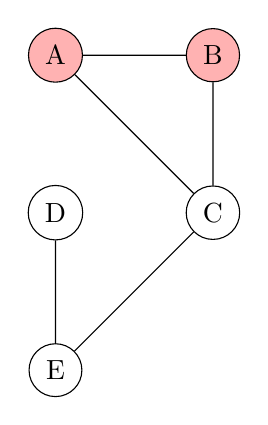
\begin{tikzpicture}[node distance=2cm]
			\node[draw, circle, fill=red!30] (A) {A};
			\node[draw, circle, fill=red!30, right of=A] (B) {B};
			\node[draw, circle, below of=B] (C) {C};
			\node[draw, circle, left of=C] (D) {D};
			\node[draw, circle, below of=D] (E) {E};

			\draw (A)--(B)--(C)--(A);
			\draw (C)--(E)--(D);
		\end{tikzpicture}
	\end{center}

\end{frame}
\begin{frame}{Step 3: $F=\{A,B,C\}$ (overflow)}

	% ---------- STEP 3 ----------
	\begin{center}

		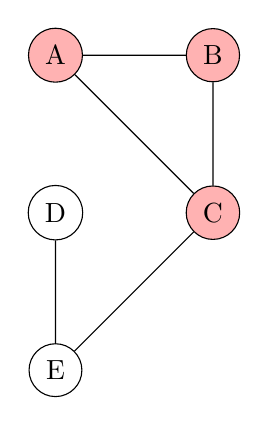
\begin{tikzpicture}[node distance=2cm]
			\node[draw, circle, fill=red!30] (A) {A};
			\node[draw, circle, fill=red!30, right of=A] (B) {B};
			\node[draw, circle, fill=red!30, below of=B] (C) {C};
			\node[draw, circle, left of=C] (D) {D};
			\node[draw, circle, below of=D] (E) {E};

			\draw (A)--(B)--(C)--(A);
			\draw (C)--(E)--(D);
		\end{tikzpicture}

	\end{center}
	\pause
	\textbf{Fix: Remove C $\Rightarrow F=\{A,B\}$}
\end{frame}

% -------- Slide 4 --------
\begin{frame}{Step 4: Add D (Overflow)}
	\begin{center}

		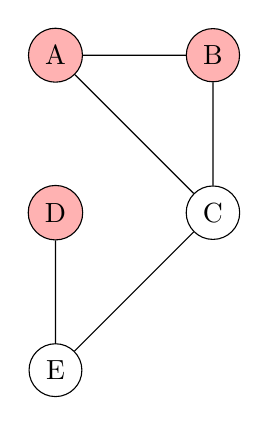
\begin{tikzpicture}[node distance=2cm]
			\node[draw, circle, fill=red!30] (A) {A};
			\node[draw, circle, fill=red!30, right of=A] (B) {B};
			\node[draw, circle, below of=B] (C) {C};
			\node[draw, circle, fill=red!30, left of=C] (D) {D};
			\node[draw, circle, below of=D] (E) {E};

			\draw (A)--(B)--(C)--(A);
			\draw (C)--(E)--(D);
		\end{tikzpicture}
	\end{center}


	\pause
	\textbf{Fix: Remove D $\Rightarrow F=\{A,B\}$}
\end{frame}

% -------- Slide 5 --------
\begin{frame}{Step 5: Add E (Overflow)}
	\begin{center}
		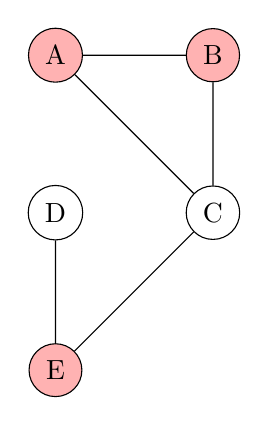
\begin{tikzpicture}[node distance=2cm]
			\node[draw, circle, fill=red!30] (A) {A};
			\node[draw, circle, fill=red!30, right of=A] (B) {B};
			\node[draw, circle, below of=B] (C) {C};
			\node[draw, circle, left of=C] (D) {D};
			\node[draw, circle, fill=red!30, below of=D] (E) {E};

			\draw (A)--(B)--(C)--(A);
			\draw (C)--(E)--(D);
		\end{tikzpicture}
	\end{center}

	\pause
	\textbf{Fix: Remove E $\Rightarrow F=\{A,B\}$}
\end{frame}

% -------- Final Slide --------
\begin{frame}{Final Answer}

	\begin{center}
		\begin{tikzpicture}[node distance=2cm]

			\node[draw, circle, below of=B] (C) {C};
			\node[draw, circle, left of=C] (D) {D};
			\node[draw, circle, below of=D] (E) {E};

			\draw (C)--(E)--(D);
		\end{tikzpicture}
	\end{center}

	\textbf{$F=\{A,B\}$}
\end{frame}






\begin{frame}{Algorithm 2: Kernelization + Bounded Search Tree}
	\begin{columns}[T]
		\column{0.48\textwidth}
		\begin{block}{Core Concept}
			\footnotesize
			Reduce graph size via preprocessing rules, then apply exact search on smaller kernel
		\end{block}

		\textbf{Reduction Rules:}
		\begin{itemize}
			\footnotesize
			\item Degree 0, 1, 2 vertices
			\item Self-loops, duplicate edges
			\item Crown decomposition
			\item Flower rule
		\end{itemize}

		\vspace{0.2cm}

		\textbf{Search Strategy:}
		\begin{itemize}
			\footnotesize
			\item Smart vertex selection
			\item Bounded depth: $k$
			\item Branching factor: $\leq 4$
		\end{itemize}

		\column{0.48\textwidth}
		\textbf{Research Directions:}
		\begin{enumerate}
			\footnotesize
			\item \textbf{New Reduction Rules}
			      \begin{itemize}
				      \scriptsize
				      \item Graph-specific rules
				      \item Theoretical contribution
			      \end{itemize}

			\item \textbf{Rule Application Order}
			      \begin{itemize}
				      \scriptsize
				      \item Optimize ordering
				      \item ML-based prediction
			      \end{itemize}

			\item \textbf{Kernelization Bounds}
			      \begin{itemize}
				      \scriptsize
				      \item Tighter bounds for special classes
				      \item Experimental validation
			      \end{itemize}

			\item \textbf{Smart Branching}
			      \begin{itemize}
				      \scriptsize
				      \item Centrality-based selection
				      \item ML-guided search
			      \end{itemize}
		\end{enumerate}

	\end{columns}
\end{frame}


\begin{frame}{Kernelization + Bounded Search Tree}
	\small
	\textbf{Idea:} Reduce the graph, then branch on remaining cycles.

	\textbf{Algorithm}
	{\small
		\setlength{\baselineskip}{8pt}
		\begin{algorithmic}[1]
			\State Apply reduction rules:
			\State \quad remove degree $\le 1$ vertices
			\State \quad contract degree-2 vertices
			\State \quad include self-loop vertices
			\State Obtain kernel $(G',k')$
			\State \textbf{function} Search$(G',k')$
			\If{$G'$ is acyclic}
			\State \textbf{return} solution
			\EndIf
			\If{$k' < 0$}
			\State \textbf{return NO}
			\EndIf
			\State find a cycle $C$
			\For{each $v \in C$}
			\State recurse on $(G' - v,\, k' - 1)$
			\EndFor
		\end{algorithmic}
	}
	\textbf{Key Insight:} Small kernel $\Rightarrow$ small search tree \\
	\textbf{Time:} $O(4^k + n^2)$
\end{frame}

%-------------------------------
% Frame 1: Original Graph
%-------------------------------
\begin{frame}{Step 1: Original Graph}
	\centering
	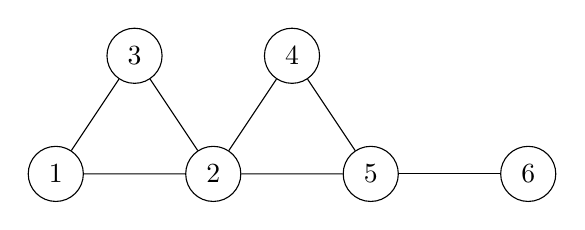
\begin{tikzpicture}[every node/.style={circle,draw,minimum size=7mm}]
		\node (1) at (0,0) {1};
		\node (2) at (2,0) {2};
		\node (3) at (1,1.5) {3};
		\node (4) at (3,1.5) {4};
		\node (5) at (4,0) {5};
		\node (6) at (6,0) {6};

		\draw (1)--(2)--(3)--(1);
		\draw (2)--(4)--(5)--(2);
		\draw (5)--(6);
	\end{tikzpicture}
\end{frame}

%-------------------------------
% Frame 2: Check degree <=1
%-------------------------------
\begin{frame}{Step 2: Remove degree $\leq$ 1 vertices}
	\centering
	\textbf{Vertex 6 removed}

	\vspace{0.5cm}

	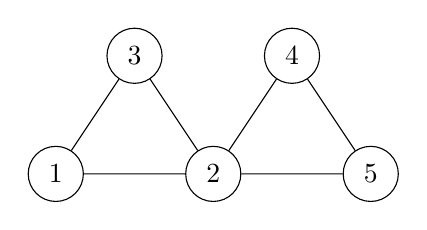
\begin{tikzpicture}[every node/.style={circle,draw,minimum size=7mm}]
		\node (1) at (0,0) {1};
		\node (2) at (2,0) {2};
		\node (3) at (1,1.5) {3};
		\node (4) at (3,1.5) {4};
		\node (5) at (4,0) {5};

		\draw (1)--(2)--(3)--(1);
		\draw (2)--(4)--(5)--(2);
	\end{tikzpicture}
\end{frame}

%-------------------------------
% Frame 3: Contract vertex 4
%-------------------------------
\begin{frame}{Step 3: Contract degree-2 vertex (4)}
	\centering
	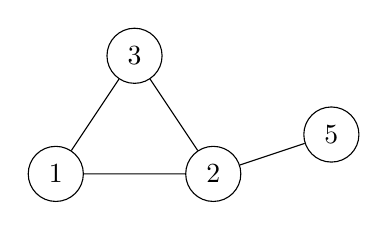
\begin{tikzpicture}[every node/.style={circle,draw,minimum size=7mm}]
		\node (1) at (0,0) {1};
		\node (2) at (2,0) {2};
		\node (3) at (1,1.5) {3};
		\node (5) at (3.5,0.5) {5};

		\draw (1)--(2)--(3)--(1);
		\draw (2)--(5);
	\end{tikzpicture}
\end{frame}

%-------------------------------
% Frame 4: Contract vertex 5
%-------------------------------
\begin{frame}{Step 4: Remove degree $\leq$ 1 vertex (5)}
	\centering
	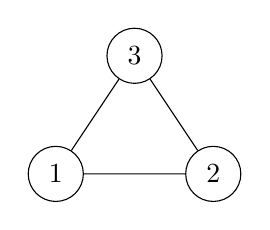
\begin{tikzpicture}[every node/.style={circle,draw,minimum size=7mm}]
		\node (1) at (0,0) {1};
		\node (2) at (2,0) {2};
		\node (3) at (1,1.5) {3};

		\draw (1)--(2)--(3)--(1);
	\end{tikzpicture}
\end{frame}

%-------------------------------
% Frame 5: Kernel obtained
%-------------------------------
\begin{frame}{Step 5: Kernel Graph (G')}
	\centering
	\textbf{Remaining cycle}

	\vspace{0.5cm}

	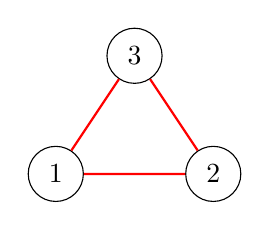
\begin{tikzpicture}[every node/.style={circle,draw,minimum size=7mm}]
		\node (1) at (0,0) {1};
		\node (2) at (2,0) {2};
		\node (3) at (1,1.5) {3};

		\draw[red, thick] (1)--(2)--(3)--(1);
	\end{tikzpicture}
\end{frame}

%-------------------------------
% Frame 6: Branch remove 1
%-------------------------------
\begin{frame}{Step 6: Branch - Remove vertex 1}
	\centering
	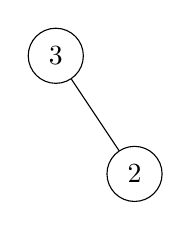
\begin{tikzpicture}[every node/.style={circle,draw,minimum size=7mm}]
		\node (2) at (2,0) {2};
		\node (3) at (1,1.5) {3};

		\draw (2)--(3);
	\end{tikzpicture}

	\vspace{0.5cm}
	Graph becomes acyclic
\end{frame}

%-------------------------------
% Frame 7: Branch remove 2
%-------------------------------
\begin{frame}{Step 7: Branch - Remove vertex 2}
	\centering
	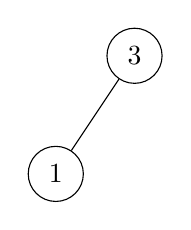
\begin{tikzpicture}[every node/.style={circle,draw,minimum size=7mm}]
		\node (1) at (0,0) {1};
		\node (3) at (1,1.5) {3};

		\draw (1)--(3);
	\end{tikzpicture}

	\vspace{0.5cm}
	Graph becomes acyclic
\end{frame}

%-------------------------------
% Frame 8: Branch remove 3
%-------------------------------
\begin{frame}{Step 8: Branch - Remove vertex 3}
	\centering
	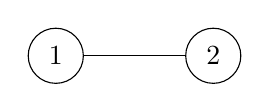
\begin{tikzpicture}[every node/.style={circle,draw,minimum size=7mm}]
		\node (1) at (0,0) {1};
		\node (2) at (2,0) {2};

		\draw (1)--(2);
	\end{tikzpicture}

	\vspace{0.5cm}
	Graph becomes acyclic
\end{frame}


\begin{frame}{Algorithm 3: Memetic Algorithm (GA + Local Search)}
	\begin{columns}[T]
		\column{0.48\textwidth}
		\begin{block}{Core Concept}
			\footnotesize
			Population evolution + local optimization for large-scale instances
		\end{block}

		\textbf{Components:}
		\begin{itemize}
			\footnotesize
			\item Smart initialization (greedy + random)
			\item FVS-aware crossover operators
			\item Centrality-based mutation
			\item Problem-specific local search
		\end{itemize}

		\vspace{0.2cm}

		\textbf{Practical Relevance:}
		\begin{itemize}
			\footnotesize
			\item Industry standard
			\item Handles $n > 1000$ vertices
			\item Near-optimal (5-10\% gap)
		\end{itemize}

		\column{0.48\textwidth}
		\textbf{Research Directions:}
		\begin{enumerate}
			\footnotesize
			\item \textbf{Cycle-Preserving Crossover}
			      \begin{itemize}
				      \scriptsize
				      \item Preserve cycle-breaking structures
				      \item Novel contribution
			      \end{itemize}

			\item \textbf{Hybrid Exact-Metaheuristic}
			      \begin{itemize}
				      \scriptsize
				      \item Use IC for small components
				      \item GA for large core
			      \end{itemize}

			\item \textbf{ML Integration}
			      \begin{itemize}
				      \scriptsize
				      \item Predict promising vertices
				      \item Learn operator selection
			      \end{itemize}

			\item \textbf{Multi-Objective}
			      \begin{itemize}
				      \scriptsize
				      \item Minimize size + maximize robustness
				      \item Pareto frontier
			      \end{itemize}
		\end{enumerate}

	\end{columns}
\end{frame}


\begin{frame}{Memetic Algorithm for FVS}
	\small
	\textbf{Idea:} Evolutionary search combined with local optimization.

	\textbf{Algorithm}
	\begin{algorithmic}[1]
		\State Encode solution as a permutation of vertices
		\State Decode by removing vertices until graph is acyclic
		\State Initialize population (greedy + random)
		\For{each generation}
		\State Evaluate fitness: $-|FVS|$
		\State Select parents (tournament)
		\State Crossover (cycle-aware)
		\State Mutation (swap cycle-heavy vertices)
		\State Local search (hill-climbing)
		\EndFor
		\State \textbf{return} best solution found
	\end{algorithmic}

	\textbf{Key Insight:} Exploration + refinement \\
	\textbf{Type:} Heuristic (near-optimal)
\end{frame}






%-------------------------------
% Frame 1: Original Graph
%-------------------------------
\begin{frame}{Step 1: Original Graph}
	\centering
	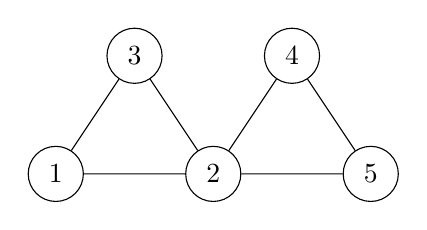
\begin{tikzpicture}[every node/.style={circle,draw,minimum size=7mm}]
		\node (1) at (0,0) {1};
		\node (2) at (2,0) {2};
		\node (3) at (1,1.5) {3};
		\node (4) at (3,1.5) {4};
		\node (5) at (4,0) {5};

		\draw (1)--(2)--(3)--(1);
		\draw (2)--(4)--(5)--(2);
	\end{tikzpicture}
\end{frame}

%-------------------------------
% Frame 2: Encoding (Permutation)
%-------------------------------
\begin{frame}{Step 2: Encode Solution}
	\centering
	Example permutation:

	\vspace{0.5cm}
	\Huge
	[3, 1, 5, 2, 4]
\end{frame}

%-------------------------------
% Frame 3: Decoding (Remove 3)
%-------------------------------
\begin{frame}{Step 3: Remove vertex 3}
	\centering
	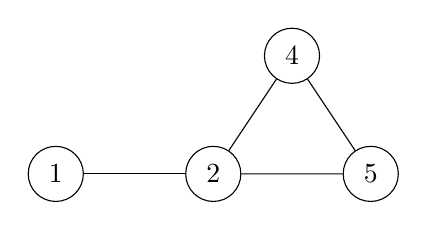
\begin{tikzpicture}[every node/.style={circle,draw,minimum size=7mm}]
		\node (1) at (0,0) {1};
		\node (2) at (2,0) {2};
		\node (4) at (3,1.5) {4};
		\node (5) at (4,0) {5};

		\draw (1)--(2);
		\draw (2)--(4)--(5)--(2);
	\end{tikzpicture}
\end{frame}

%-------------------------------
% Frame 4: Remove 1
%-------------------------------
\begin{frame}{Step 4: Remove vertex 1}
	\centering
	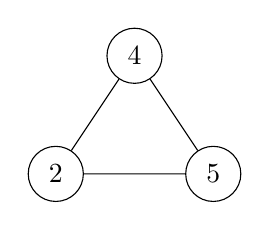
\begin{tikzpicture}[every node/.style={circle,draw,minimum size=7mm}]
		\node (2) at (2,0) {2};
		\node (4) at (3,1.5) {4};
		\node (5) at (4,0) {5};

		\draw (2)--(4)--(5)--(2);
	\end{tikzpicture}
\end{frame}


%-------------------------------
% Frame 5: Remove 5 (graph becomes acyclic)
%-------------------------------
\begin{frame}{Step 5: Remove vertex 5}
	\centering
	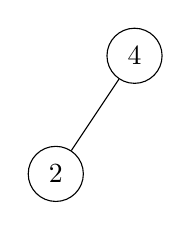
\begin{tikzpicture}[every node/.style={circle,draw,minimum size=7mm}]
		\node (2) at (2,0) {2};
		\node (4) at (3,1.5) {4};

		\draw (2)--(4);
	\end{tikzpicture}

	\vspace{0.5cm}
	Graph is now acyclic $\rightarrow$ Stop decoding
\end{frame}

%-------------------------------
% Frame 6: Fitness Evaluation
%-------------------------------
\begin{frame}{Step 6: Fitness Evaluation}
	\centering
	Removed vertices = \{3,1,5\}

	\vspace{0.5cm}
	Fitness = $-|FVS| = -3$
\end{frame}

%-------------------------------
% Frame 7: Selection
%-------------------------------
\begin{frame}{Step 7: Selection (Tournament)}
	\centering
	Select best solutions from population

	\vspace{0.5cm}
	Example:
	\[
		[3,1,5,2,4],\quad [2,4,1,5,3]
	\]
\end{frame}

%-------------------------------
% Frame 8: Crossover
%-------------------------------
\begin{frame}{Step 8: Crossover}
	\centering
	Parent 1: [3,1,5,2,4]

	Parent 2: [2,4,1,5,3]

	\vspace{0.5cm}
	Child:

	\Huge
	[3,4,1,2,5]
\end{frame}

%-------------------------------
% Frame 9: Mutation
%-------------------------------
\begin{frame}{Step 9: Mutation}
	\centering
	Before:

	\[
		[3,4,1,2,5]
	\]

	\vspace{0.5cm}
	After swap:

	\Huge
	[3,1,4,2,5]
\end{frame}

%-------------------------------
% Frame 10: Local Search
%-------------------------------
\begin{frame}{Step 10: Local Search}
	\centering
	Try improving solution:

	\vspace{0.5cm}
	Remove fewer vertices if possible

	\vspace{0.5cm}
	Example improvement:

	\Huge
	FVS size: 3 $\rightarrow$ 2
\end{frame}

%-------------------------------
% Frame 11: Final Solution
%-------------------------------
\begin{frame}{Step 11: Best Solution}
	\centering
	Best FVS found:

	\vspace{0.5cm}
	\Huge
	\{3,2\}

	\vspace{0.5cm}
	Graph becomes acyclic
\end{frame}






% ════════════════════════════════════════════════════════════════════════════
\section{Our Modifications}

\begin{frame}[plain]
	\centering
	\vspace{1.2cm}
	{\Huge \textbf{Our Modifications}}\\[8pt]
	{\Large KMA \quad DKMA \quad GNN-KMA}
\end{frame}

% ════════════════════════════════════════════════════════════════════════════
\subsection{KMA: Kernelized Memetic Algorithm}

\begin{frame}{KMA - Motivation and High-Level Design}
	\begin{columns}[T]
		\begin{column}{0.52\textwidth}
			\textbf{Why not pure Memetic Algorithm?}
			\begin{itemize}
				\item A plain MA \cite{lust2010} operates on the full graph
				\item Reduction rules can \emph{safely} eliminate many vertices
				      before any search \cite{thomasse2010}
				\item This shrinks the search space, letting MA focus on hard subgraphs
			\end{itemize}
			\vspace{6pt}
			\textbf{KMA Pipeline}
			\begin{enumerate}\setlength\itemsep{2pt}
				\item \highlight{Kernelization} - apply reduction rules, record forced vertices
				\item \highlight{MA on kernel} - C++ evolutionary search on reduced graph
				\item \highlight{Reconstruction} - map kernel solution to original indices,
				      union with forced vertices
			\end{enumerate}
		\end{column}
		\begin{column}{0.44\textwidth}
			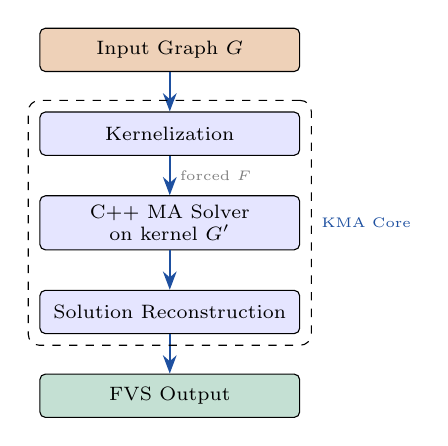
\begin{tikzpicture}[
					node distance=0.5cm,
					block/.style={draw,rounded corners=2pt,fill=blue!10,
							minimum width=3.3cm,minimum height=0.55cm,
							font=\scriptsize,align=center},
					arr/.style={->,>=Stealth,thick,midblue}]
				\node[block,fill=warnorange!30] (in)   {Input Graph $G$};
				\node[block,below=of in]  (kern) {Kernelization};
				\node[block,below=of kern](ma)   {C++ MA Solver\\on kernel $G'$};
				\node[block,below=of ma]  (recon){Solution Reconstruction};
				\node[block,below=of recon,fill=successgreen!25] (out) {FVS Output};
				\draw[arr] (in)--(kern);
				\draw[arr] (kern)--(ma) node[midway,right,font=\tiny,text=gray]
				{forced $F$};
				\draw[arr] (ma)--(recon);
				\draw[arr] (recon)--(out);
				\node[draw,dashed,rounded corners,fit=(kern)(ma)(recon),
					inner sep=4pt,label={[font=\tiny,midblue]right:KMA Core}]{};
			\end{tikzpicture}
		\end{column}
	\end{columns}
\end{frame}

\begin{frame}{KMA - Kernelization Rules}
	\begin{columns}[T]
		\begin{column}{0.47\textwidth}
			\begin{block}{Undirected Kernelization Rules}
				\begin{enumerate}\setlength\itemsep{3pt}
					\item \textbf{Self-loop:} vertex with self-loop $\Rightarrow$ force into FVS
					\item \textbf{Degree-0/1:} acyclic leaf $\Rightarrow$ safely delete
					\item \textbf{Degree-2 bypass:} if $\deg(v)=2$ with neighbors $a,b$
					      and $\{a,b\}\notin E$:
					      delete $v$, add edge $(a,b)$
				\end{enumerate}
				Rules applied \textbf{iteratively} until quiescence.\\[4pt]
				Theoretical basis: $O(k^2)$ kernel \cite{thomasse2010}.
			\end{block}
		\end{column}
		\begin{column}{0.47\textwidth}
			\begin{block}{Directed Kernelization Rules}
				\begin{enumerate}\setlength\itemsep{3pt}
					\item \textbf{Self-loop:} forced into DFVS
					\item \textbf{Source/Sink:} $\text{in-deg}=0$ or $\text{out-deg}=0$
					      $\Rightarrow$ delete (not on any directed cycle)
					\item \textbf{Degree-1 bypass:} in-deg or out-deg $=1$
					      $\Rightarrow$ shortcut edges, delete vertex
					\item \textbf{SCC reduction:} retain only vertices in
					      nontrivial SCCs (size $>1$ or self-loop)
				\end{enumerate}
				Directed kernel theory: \cite{chen2008dfvs}.
			\end{block}
		\end{column}
	\end{columns}
	\vspace{4pt}
	\begin{tcolorbox}[greenbox,fontupper=\footnotesize]
		\textbf{Modification over baseline MA:} The addition of kernelization
		(especially the SCC-based directed reduction) is a key novelty.
		SCC reduction alone can eliminate \textbf{60--90\%} of vertices
		on sparse real-world directed graphs before any search begins.
	\end{tcolorbox}
\end{frame}

\begin{frame}{KMA - Memetic Algorithm Core}
	\begin{columns}[T]
		\begin{column}{0.50\textwidth}
			\textbf{C++ MA Solver} (evolutionary search on kernel):
			\begin{itemize}\setlength\itemsep{2pt}
				\item Initialise population of size $P$ randomly
				\item Each individual: binary vector over kernel vertices
				\item Each generation:
				      \begin{enumerate}\setlength\itemsep{1pt}
					      \item \textbf{Crossover} (two parents $\to$ offspring)
					      \item \textbf{Local mutation} (flip, swap)
					      \item \textbf{Repair}: restore FVS validity via greedy cycle cover
					      \item \textbf{Selection}: tournament
				      \end{enumerate}
				\item Early-stop if no improvement for $T$ generations
				\item Hard wall-clock timeout enforced inside C++
			\end{itemize}
			\vspace{4pt}
			Solver dispatch priority (best-first):
			\texttt{KMA} $\to$ \texttt{KME} $\to$ \texttt{MA}
		\end{column}
		\begin{column}{0.50\textwidth}
			\begin{block}{Parameters}
				\begin{tabular}{lll}
					\toprule
					Param           & Flag                 & Default \\
					\midrule
					Population      & \texttt{--pop}       & 20      \\
					Max generations & \texttt{--gens}      & 100     \\
					Timeout         & \texttt{--timeout}   & 600s    \\
					Early-stop      & \texttt{--earlystop} & 30      \\
					\bottomrule
				\end{tabular}
			\end{block}
			\vspace{6pt}
			\begin{tcolorbox}[algbox,title=Complexity Note]
				\footnotesize
				Kernelization: $O(n+m)$ per pass\\
				MA on kernel $G'$: heuristic,\\
				~~$O(P \cdot \text{gen} \cdot |V(G')|)$\\
				Full pipeline: practical for\\
				~~$|V| \le 10^4$ within timeout
			\end{tcolorbox}
		\end{column}
	\end{columns}
\end{frame}

% ════════════════════════════════════════════════════════════════════════════
\subsection{DKMA: Dynamic Kernelized Memetic Algorithm}
% ════════════════════════════════════════════════════════════════════════════

\begin{frame}{DKMA - Dynamic Kernelized Memetic Algorithm - Core Idea}
	\begin{columns}[T]
		\begin{column}{0.52\textwidth}
			\textbf{Limitation of static kernelization (KMA):}
			\begin{itemize}
				\item Kernelization is applied \emph{once} before MA
				\item Partial solutions during MA may \emph{unlock} new reductions -
				      these are never exploited
			\end{itemize}
			\vspace{4pt}
			\textbf{DKMA - Dynamic interleaving} \cite{pace2022,esa2022}:
			\begin{enumerate}\setlength\itemsep{2pt}
				\item Evolve population for one MA generation
				\item \highlight{Commit} vertices appearing in $\ge \tau$ fraction of individuals
				\item Force committed vertices into the solution
				\item \highlight{Re-kernelize} residual graph
				\item Continue MA on the smaller kernel
			\end{enumerate}
			\vspace{4pt}
			This \textbf{opening-up effect} progressively shrinks the kernel
			as partial agreement is reached.
		\end{column}
		\begin{column}{0.44\textwidth}
			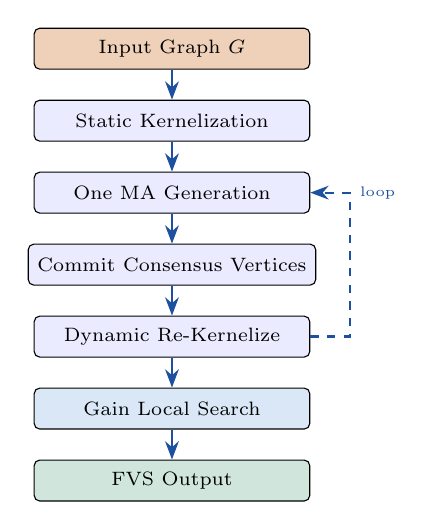
\begin{tikzpicture}[
					node distance=0.38cm,
					block/.style={draw,rounded corners=2pt,fill=blue!8,
							minimum width=3.5cm,minimum height=0.52cm,
							font=\scriptsize,align=center},
					loopback/.style={->,>=Stealth,thick,midblue,dashed},
					arr/.style={->,>=Stealth,thick,midblue}]
				\node[block,fill=warnorange!30] (in)   {Input Graph $G$};
				\node[block,below=of in]  (k1)   {Static Kernelization};
				\node[block,below=of k1]  (gen)  {One MA Generation};
				\node[block,below=of gen] (cmt)  {Commit Consensus Vertices};
				\node[block,below=of cmt] (rk)   {Dynamic Re-Kernelize};
				\node[block,below=of rk,fill=accentblue!20]  (ls)   {Gain Local Search};
				\node[block,below=of ls,fill=successgreen!20] (out) {FVS Output};
				\draw[arr] (in)--(k1);
				\draw[arr] (k1)--(gen);
				\draw[arr] (gen)--(cmt);
				\draw[arr] (cmt)--(rk);
				\draw[loopback] (rk.east) -- ++(0.5,0) |- (gen.east)
				node[midway,right,font=\tiny,text=midblue]{loop};
				\draw[arr] (rk)--(ls);
				\draw[arr] (ls)--(out);
			\end{tikzpicture}
		\end{column}
	\end{columns}
\end{frame}

\begin{frame}{DKMA - Key Innovations \& Helpers}
	\tiny
	\begin{columns}[T]
		\begin{column}{0.47\textwidth}
			\begin{block}{SHORTONE Directed Contractions}
				Inspired by the Mount-Doom PACE 2022 solver \cite{langedal2022},
				a directed contraction pass (\texttt{\_apply\_shortone\_rule})
				is applied before the MA loop on directed graphs.\\[3pt]
				Contracts degree-1 in/out vertices with special cycle-preserving rewiring,
				enabling additional SCC reductions.
			\end{block}
			\vspace{4pt}
			\begin{block}{Topological Diversification}
				Every 5 generations, \texttt{\_diversify\_with\_topological\_ordering}
				is called:\\
				\begin{itemize}
					\item Directed: randomised Kahn's algorithm tie-breaking
					\item Undirected: random spanning-tree cycle-breaking insertion
				\end{itemize}
				Prevents premature convergence \cite{lust2010}.
			\end{block}
		\end{column}
		\begin{column}{0.47\textwidth}
			\begin{block}{Gain Local Search (post-loop)}
				\texttt{\_gain\_local\_search} applies \textbf{1-1} and \textbf{2-1}
				improvement swaps after the MA loop:
				\begin{itemize}
					\item \textbf{1-1 swap}: remove one FVS vertex, add another
					      if acyclicity is preserved and size decreases
					\item \textbf{2-1 swap}: replace two FVS vertices with one
				\end{itemize}
			\end{block}
			\vspace{4pt}
			\begin{block}{Commit Threshold \& Cap}
				\texttt{\_commit\_vertices\_from\_population}:
				\begin{itemize}
					\item Commit if vertex appears in $\ge \tau$ of population
					\item Cap at top 30\% by frequency if over-committing
					\item Default $\tau = 0.8$
				\end{itemize}
				Based on DFVS IPEC 2022 approach \cite{pace2022}.
			\end{block}
		\end{column}
	\end{columns}
\end{frame}

\begin{frame}{DKMA - Correctness \& Comparison with KMA}
	\small
	\begin{columns}[T]
		\begin{column}{0.44\textwidth}
			\begin{block}{Correctness Safeguards}
				\begin{itemize}\setlength\itemsep{2pt}
					\item Deduplicated final solution indices
					\item All forced vertices (static + dynamic) included
					\item Final \textbf{acyclicity verification} on original graph:
					      directed $\Rightarrow$ iterative DFS back-edge detection;\\
					      undirected $\Rightarrow$ union-find cycle check
					\item \red{Fallback to KMA} if validation fails
				\end{itemize}
			\end{block}
		\end{column}
		\begin{column}{0.52\textwidth}
			\begin{block}{KMA vs DKMA - Key Differences}
				\begin{tabular}{p{2.6cm}p{2.0cm}p{2.0cm}}
					\toprule
					Feature          & KMA  & DKMA           \\
					\midrule
					Kernelization    & Once & Per loop       \\
					Commitment       & None & Consensus      \\
					SHORTONE pass    & No   & Yes (directed) \\
					Topological div. & No   & Every 5 gen.   \\
					Local search     & No   & Gain 1-1/2-1   \\
					Acyclicity check & End  & End + fallback \\
					\bottomrule
				\end{tabular}
			\end{block}
		\end{column}
	\end{columns}
	\vspace{4pt}
	\begin{tcolorbox}[orangebox,fontupper=\footnotesize]
		\textbf{References:} DKMA design is inspired by the PACE 2022 FVS track
		winner strategies \cite{pace2022} (Grossmann, Heuer, Schulz, Strash, IPEC 2022)
		and the ESA 2022 DFVS analysis \cite{esa2022}
		(Figiel, Froese, Nichterlein, Niedermeier).
		The Mount-Doom SHORTONE rule is from Langedal et al.\ \cite{langedal2022}.
	\end{tcolorbox}
\end{frame}

% ════════════════════════════════════════════════════════════════════════════
\subsection{GNN-KMA Models}
% ════════════════════════════════════════════════════════════════════════════

\begin{frame}{GNN-KMA - Hybrid Coupling Strategy}
	\tiny
	\begin{columns}[T]
		\begin{column}{0.50\textwidth}
			\textbf{Motivation:}
			\begin{itemize}
				\item GNN learns vertex-level patterns from solved instances
				\item Predicts probability $p(v)$ of belonging to FVS
				\item High-confidence predictions \textbf{hard-fix} vertices
				      before KMA, reducing the search problem
			\end{itemize}
			\vspace{6pt}
			\textbf{Precision-first soft-hint coupling:}
			\begin{enumerate}\setlength\itemsep{2pt}
				\item Kernelize graph $G \to G'$
				\item Run GNN on $G'$, get $p(v)$ for each $v$
				\item Hard-fix only vertices with $p(v) \ge \theta$
				\item Cap hard-fix at \textbf{8\%} of kernel size
				\item Run KMA on residual kernel
				\item Reconstruct: forced $\cup$ GNN-fixed $\cup$ KMA output
			\end{enumerate}
			\vspace{3pt}
			{\footnotesize Default: $\theta=0.65$,
				min-fix $= 0.5\%$, max-fix $= 8\%$ of kernel}
		\end{column}
		\begin{column}{0.46\textwidth}
			\begin{tcolorbox}[mybox,title=Why Precision-First?]
				\footnotesize
				False positives in hard-fixing are \textbf{catastrophic}:
				a wrongly fixed vertex inflates the FVS size permanently
				within that branch. Capping at 8\% and requiring $\theta \ge 0.65$
				ensures the GNN only commits when highly confident.
				\\[4pt]
				If no vertex exceeds $\theta$, the system
				\textbf{falls back to pure KMA} automatically.
			\end{tcolorbox}
			\vspace{5pt}
			\begin{tcolorbox}[greenbox,fontupper=\footnotesize]
				\textbf{Can you do a GNN-DKMA variant?} Same coupling, but
				the residual kernel is handed to DKMA instead of KMA,
				enabling dynamic re-kernelization atop GNN guidance.
			\end{tcolorbox}
		\end{column}
	\end{columns}
\end{frame}

% ─── GNN-KMA v1 ───────────────────────────────────────────────────────────────
\begin{frame}{GNN-KMA v1 - Baseline Architecture}
	\tiny
	\begin{columns}[T]
		\begin{column}{0.47\textwidth}
			\begin{block}{Feature Engineering (3 channels)}
				\textbf{Undirected:}
				\begin{itemize}
					\item Normalised degree $d(v)/d_{\max}$
					\item Clustering coefficient $c(v)$ \cite{watts1998}
					\item Normalised $\log$-degree
				\end{itemize}
				\textbf{Directed:}
				\begin{itemize}
					\item Normalised in-degree
					\item Normalised out-degree
					\item Normalised $\min(\text{in},\text{out})$-degree
				\end{itemize}
			\end{block}
			\vspace{4pt}
			\begin{tcolorbox}[algbox,title=Design Choice]
				\footnotesize
				Clustering coefficient \cite{watts1998} captures local cycle density -
				vertices with high $c(v)$ are strong FVS candidates.
				This is a well-established heuristic from the
				small-world network literature.
			\end{tcolorbox}
		\end{column}
		\begin{column}{0.47\textwidth}
			\begin{block}{Model Architecture}
				\textbf{UndirectedFVSNet:}
				\begin{itemize}
					\item 3-layer \textbf{GraphSAGE} message passing \cite{hamilton2017}
					\item BatchNorm + Dropout after each layer
					\item MLP classification head
					\item 2-class \texttt{log-softmax} output
				\end{itemize}
				\textbf{DirectedFVSNet:}
				\begin{itemize}
					\item Custom directed aggregation layer\\
					      (separate in / out / self terms)
					\item 3 layers + BN + Dropout + MLP
					\item 2-class \texttt{log-softmax} output
				\end{itemize}
			\end{block}
			\vspace{2pt}
			\begin{block}{Training Objective}
				Weighted NLL loss $+$ cosine LR schedule.\\
				Checkpoint by \textbf{validation F1} score.
			\end{block}
		\end{column}
	\end{columns}
	\vspace{2pt}
	{\scriptsize\color{gray}
		GraphSAGE \cite{hamilton2017}: Hamilton et al., NeurIPS 2017.}
\end{frame}

% ─── GNN-KMA v2 ───────────────────────────────────────────────────────────────
\begin{frame}{GNN-KMA v2 - Richer Structural Features}
	\tiny
	\begin{columns}[T]
		\begin{column}{0.47\textwidth}
			\begin{block}{Feature Engineering (11 channels)}
				\begin{enumerate}\setlength\itemsep{2pt}
					\item Degree-like channels (in/out/min or undirected)
					\item \textbf{RWSE} - Random Walk Structural Encoding
					      \cite{dwivedi2021}\\
					      {\footnotesize short-range return probabilities at steps
					      $\{2,3,4\}$}
					\item \textbf{Motif counts}: triangle count,
					      4-cycle participation, 4-clique style counts \cite{ahmed2015}
					\item \textbf{k-core number} $\kappa(v)$ \cite{batagelj2003}
				\end{enumerate}
			\end{block}
		\end{column}
		\begin{column}{0.47\textwidth}
			\begin{block}{Architecture \& Training}
				\textbf{UndirectedFVSNetV2 / DirectedFVSNetV2:}
				\begin{itemize}
					\item Same GraphSAGE-style backbone as v1
					\item Upgraded input: \texttt{in\_channels=11}
					\item Richer representation $\Rightarrow$ stronger
					      structural discrimination
				\end{itemize}
				\vspace{4pt}
				\textbf{Training:} same NLL + cosine schedule;
				checkpoint by validation F1.
			\end{block}
			\vspace{4pt}
			\begin{tcolorbox}[algbox,title=Why These Features?]
				\footnotesize
				\textbf{RWSE} \cite{dwivedi2021}: captures short-range cycle
				return probability - directly relevant to FVS membership.\\[3pt]
				\textbf{k-core} \cite{batagelj2003}: vertices deep in dense
				cores are more likely to be in any FVS.\\[3pt]
				\textbf{Motif counts} \cite{ahmed2015}: triangle/4-cycle
				participation indicates cycle exposure.
			\end{tcolorbox}
		\end{column}
	\end{columns}
\end{frame}

% ─── GNN-KMA v3 ───────────────────────────────────────────────────────────────
\begin{frame}{GNN-KMA v3 - Attention-Based Precision Model}
	\tiny
	\begin{columns}[T]
		\begin{column}{0.47\textwidth}
			\begin{block}{Feature Engineering (16 channels)}
				\begin{itemize}\setlength\itemsep{2pt}
					\item Extended \textbf{RWSE} horizon: steps $\{2,3,4,6,8,12,16\}$
					      \cite{dwivedi2021}
					\item \textbf{SCC-aware channels} for directed cycle structure
					      (SCC size, SCC membership depth)
					\item Cycle-score interaction features
					\item Directional ratio features ($\text{in}/(\text{in}+\text{out})$)
					\item Reduced reliance on expensive motif channels
				\end{itemize}
			\end{block}
			\vspace{3pt}
			\begin{tcolorbox}[algbox,title=SCC Channels (Directed)]
				\footnotesize
				SCC decomposition \cite{tarjan1972} provides structural depth:
				vertices in large SCCs are more critical for DFVS.
				SCC-size and SCC-depth channels directly encode this.
			\end{tcolorbox}
		\end{column}
		\begin{column}{0.47\textwidth}
			\begin{block}{DirectedFVSNetV3 Architecture}
				\begin{itemize}\setlength\itemsep{2pt}
					\item Input projection layer
					\item \textbf{5 residual GATv2 blocks} \cite{brody2022}
					\item Separate \textbf{forward} and \textbf{reverse} message paths
					\item Per-layer fusion projections
					\item \textbf{Global readout context} concatenated to node embedding
					\item Single-logit output per node (sigmoid)
				\end{itemize}
			\end{block}
			\vspace{3pt}
			\begin{block}{v3 Training Innovations}
				\begin{itemize}
					\item \textbf{AsymmetricFVSLoss}: penalises false positives more
					      strongly (precision-oriented)
					\item Warmup + cosine LR + \textbf{gradient clipping}
					\item Checkpoint metric: \textbf{topk-precision@8\%}
					      (matches hard-fix cap)
					\item 200 epochs (vs 100 for v1/v2)
				\end{itemize}
			\end{block}
		\end{column}
	\end{columns}
\end{frame}

\begin{frame}{GNN-KMA - Feature \& Architecture Evolution Summary}
	\small
	\begin{center}
		\begin{tabular}{llll}
			\toprule
			\textbf{Aspect}                     & \textbf{v1}                   & \textbf{v2}       & \textbf{v3}            \\
			\midrule
			Feature channels                    & 3                             & 11                & 16                     \\
			Degree features                     & \checkmark                    & \checkmark        & \checkmark             \\
			Clustering coeff.\ \cite{watts1998} & \checkmark                    & --                & --                     \\
			RWSE \cite{dwivedi2021}             & --                            & steps $\{2,3,4\}$ & steps $\{2..16\}$      \\
			Motif counts \cite{ahmed2015}       & --                            & \checkmark        & reduced                \\
			k-core \cite{batagelj2003}          & --                            & \checkmark        & --                     \\
			SCC channels \cite{tarjan1972}      & --                            & --                & \checkmark             \\
			Backbone                            & GraphSAGE \cite{hamilton2017} & GraphSAGE         & GATv2 \cite{brody2022} \\
			Depth                               & 3 layers                      & 3 layers          & 5 residual blocks      \\
			Bidirectional                       & No                            & No                & Yes (fwd+rev)          \\
			Global readout                      & No                            & No                & Yes                    \\
			Loss                                & NLL                           & NLL               & AsymmetricFVSLoss      \\
			Checkpoint metric                   & Val F1                        & Val F1            & topk-prec@8\%          \\
			Epochs                              & 100                           & 100               & 200                    \\
			\bottomrule
		\end{tabular}
	\end{center}
\end{frame}

% ════════════════════════════════════════════════════════════════════════════
\section{Results}
% ════════════════════════════════════════════════════════════════════════════
\begin{frame}[plain]
	\centering
	\vspace{1.0cm}
	{\Huge \textbf{Results}}\\[6pt]
	{\Large Synthetic Dataset \quad PACE 2022 \quad Evaluation}
\end{frame}

\begin{frame}{Notation \& Terms}
	\begin{itemize}
		\item \textbf{MA}: Memetic Algorithm - a genetic algorithm with local search
		\item \textbf{KMA}: Kernelized Memetic Algorithm - MA applied on a reduced kernel
		\item \textbf{DKMA}: Dynamic Kernelized Memetic Algorithm - KMA with iterative re-kernelization
		\item \textbf{GNN-KMA}: GNN-augmented KMA - GNN guides/fixes high-confidence vertices for KMA
	\end{itemize}
\end{frame}

\subsection{Synthetic Dataset}

\begin{frame}{Dataset - Design Goals \& Generation Pipeline}
	\tiny
	\begin{columns}[T]
		\begin{column}{0.52\textwidth}
			\textbf{Five design goals:}
			\begin{enumerate}\setlength\itemsep{2pt}
				\item \highlight{Controlled distribution} - fixed category proportions
				\item \highlight{Track-aware difficulty} - separate exact \& heuristic tracks
				\item \highlight{Reproducibility} - deterministic seeding throughout
				\item \highlight{Restartability} - safe reuse of existing files
				\item \highlight{Benchmark/train alignment} - PT datasets mirror
				      TXT corpus structure
			\end{enumerate}
			\vspace{6pt}
			\textbf{Three-stage orchestration:}
			\begin{enumerate}
				\item \texttt{download\_real\_world.py}\\
				      {\footnotesize NetworkX, PyG, OGB, SNAP sources}
				\item \texttt{generate\_synthetic.py}\\
				      {\footnotesize Barabási–Albert, Watts–Strogatz, ER, grids, trees, DAGs}
				\item \texttt{dataset\_gen.py}\\
				      {\footnotesize TXT $\to$ PyG Data objects with solver labels}
			\end{enumerate}
		\end{column}
		\begin{column}{0.44\textwidth}
			\begin{tcolorbox}[mybox,title=Directory Contract]
				\footnotesize
				\texttt{data/synthetic/}\\
				\quad\texttt{\{undirected|directed\}/}\\
				\quad\quad\texttt{\{exact\_track|heuristic\_track\}/}\\
				\quad\quad\quad\texttt{\{category\}/}\\
				\quad\quad\quad\quad\texttt{*.txt}
			\end{tcolorbox}
			\vspace{6pt}
			\begin{block}{Track Size Intent}
				\begin{tabular}{ll}
					\toprule
					Track            & Node range                  \\
					\midrule
					exact\_track     & $\approx 10$--$35$ nodes    \\
					heuristic\_track & $\approx 100$--$5000$ nodes \\
					\bottomrule
				\end{tabular}
			\end{block}
			\vspace{4pt}
			\begin{tcolorbox}[greenbox,fontupper=\footnotesize]
				\textbf{Default:} 100K undirected + 100K directed\\
				exact ratio = 0.5, seed = 1337
			\end{tcolorbox}
		\end{column}
	\end{columns}
\end{frame}

\begin{frame}{Dataset - Undirected Distribution}
	\small
	\begin{block}{Undirected Categories (20\% each)}
		\begin{tabular}{lll}
			\toprule
			Category              & Weight & Graph Model                         \\
			\midrule
			\texttt{real\_world}  & 20\%   & NetworkX/PyG/OGB/SNAP               \\
			\texttt{scale\_free}  & 20\%   & Barabási–Albert \cite{barabasi1999} \\
			\texttt{small\_world} & 20\%   & Watts–Strogatz \cite{watts1998}     \\
			\texttt{random\_er}   & 20\%   & Erdős–Rényi \cite{erdos1959}        \\
			\texttt{grids\_trees} & 20\%   & Grid + Random tree                  \\
			\bottomrule
		\end{tabular}
	\end{block}
	\vspace{0.3cm}
	\begin{tcolorbox}[greenbox,fontupper=\footnotesize]
		\textbf{Note:} The undirected dataset balances real-world graphs,
		scale-free networks, small-world models, random Erdős–Rényi graphs,
		and structured grids/trees.
	\end{tcolorbox}
\end{frame}

\begin{frame}{Dataset - Directed Distribution}
	\small
	\begin{block}{Directed Categories}
		\begin{tabular}{ll}
			\toprule
			Category                  & Weight \\
			\midrule
			\texttt{real\_world\_ego} & 30\%   \\
			\texttt{scale\_free}      & 20\%   \\
			\texttt{random\_er}       & 20\%   \\
			\texttt{directed\_grids}  & 15\%   \\
			\texttt{dags}             & 15\%   \\
			\bottomrule
		\end{tabular}
	\end{block}
	\vspace{0.3cm}
	\begin{tcolorbox}[greenbox,fontupper=\footnotesize]
		\textbf{Note:} Directed instances include ego-networks,
		scale-free digraphs, random directed graphs, grid-based graphs,
		and acyclic DAG structures.
	\end{tcolorbox}
\end{frame}

\begin{frame}{Dataset - Real-World Share \& Labels}
	\small
	\begin{columns}[T]
		\begin{column}{0.50\textwidth}
			\begin{tcolorbox}[greenbox,fontupper=\footnotesize]
				\textbf{Real-world share:}\\
				Undirected: 20\% real-world graphs\\
				Directed: 30\% ego-network graphs\\[3pt]
				Sources: NetworkX built-ins, PyG datasets,
				OGB node property datasets, SNAP archives.\\[3pt]
				Cached under \texttt{.cache/real\_graphs}.
			\end{tcolorbox}
		\end{column}
		\begin{column}{0.46\textwidth}
			\begin{tcolorbox}[algbox,title=Label Sources]
				\footnotesize
				\textbf{exact\_track}: IC solver labels\\
				(high-fidelity, near-optimal)\\[3pt]
				\textbf{heuristic\_track}: KMA labels\\
				(practical, large-instance behavior)
			\end{tcolorbox}
		\end{column}
	\end{columns}
\end{frame}

\begin{frame}{Dataset - Why We Used This Approach}
	\tiny
	\begin{columns}[T]
		\begin{column}{0.46\textwidth}
			\begin{block}{Diversity}
				\begin{itemize}\setlength\itemsep{2pt}
					\item \textbf{5 undirected families}: covers scale-free hubs,
					      small-world clusters, random structure,
					      regular grids/trees, and real topology
					\item \textbf{5 directed families}: adds ego networks and DAGs
					\item Both undirected and directed instances
					\item Two difficulty regimes (exact / heuristic)
				\end{itemize}
			\end{block}
			\vspace{4pt}
			\begin{block}{Scale}
				100K total undirected + 100K directed\\
				{\footnotesize (20K version also available on Kaggle)}\\[4pt]
				Largest publicly available FVS dataset
				with ground-truth labels to our knowledge.
			\end{block}
		\end{column}
		\begin{column}{0.50\textwidth}
			\begin{block}{Quality Guarantees}
				\begin{itemize}\setlength\itemsep{2pt}
					\item Each label validated via acyclicity check
					\item Subprocess timeout isolation for all solver calls
					\item CSV status ledger tracks
					      completed / timeout / invalid outcomes
					\item Largest connected component extracted
					\item Compact integer relabelling applied
					\item No self-loops in edge lists
				\end{itemize}
			\end{block}
			\vspace{4pt}
			\begin{tcolorbox}[greenbox,fontupper=\footnotesize]
				\faDatabase~\textbf{Kaggle (100K):}\\
				\href{https://www.kaggle.com/datasets/tawkirazizrahman/fvs-synthetic-dataset-100k}{%
					\texttt{kaggle.com/.../fvs-synthetic-dataset-100k}}\\[4pt]
				\faDatabase~\textbf{Kaggle (20K):}\\
				\href{https://www.kaggle.com/datasets/tawkirazizrahman/fvs-synthetic-dataset-20k}{%
					\texttt{kaggle.com/.../fvs-synthetic-dataset-20k}}
			\end{tcolorbox}
		\end{column}
	\end{columns}
\end{frame}

% ════════════════════════════════════════════════════════════════════════════
\subsection{PACE 2022 Benchmark}
% ════════════════════════════════════════════════════════════════════════════

\begin{frame}{PACE 2022 Dataset - Real-World Benchmark Testing}
	\tiny
	\begin{columns}[T]
		\begin{column}{0.52\textwidth}
			\begin{block}{What is PACE 2022?}
				The \textbf{Parameterized Algorithms and Computational Experiments}
				(PACE) Challenge 2022 \cite{pace2022} focused on the
				\textbf{Feedback Vertex Set} problem.\\[5pt]
				It provided:
				\begin{itemize}
					\item 200 public undirected test instances
					\item Curated from real-world and synthetic sources
					\item Difficulty ranges from small exact to large heuristic
					\item Official solution checker for validation
					\item World-class solver implementations as baselines
				\end{itemize}
			\end{block}
		\end{column}
		\begin{column}{0.44\textwidth}
			\begin{block}{Usage in This Project}
				\begin{itemize}\setlength\itemsep{3pt}
					\item PACE 2022 instances stored under
					      \texttt{data/pace2022/}
					\item \textbf{Protected from cleanup} - never deleted
					      by \texttt{setup\_benchmark\_inputs.py}
					\item Benchmarked via \texttt{pacerun.sh}
					      and \texttt{paceresults/}
					\item Used to evaluate \textbf{heuristic solvers}
					      (KMA, DKMA, GNN-KMA v1/v2/v3)
					      against real competition-grade instances
					\item PACE winner results in \texttt{pace2022\_winner.csv}
					      used as comparison baseline
				\end{itemize}
			\end{block}
		\end{column}
	\end{columns}
	\vspace{4pt}
	\begin{tcolorbox}[orangebox,fontupper=\footnotesize]
		\textbf{Why PACE 2022?} Our synthetic dataset covers diverse graph families
		but may not capture the nuances of competition-curated real-world instances.
		PACE 2022 instances serve as a \emph{held-out real-world stress test}
		for heuristic solvers, enabling direct comparison with state-of-the-art
		PACE competitors \cite{pace2022}.
	\end{tcolorbox}
\end{frame}


\begin{frame}{End-to-End System Architecture}
	\begin{center}
		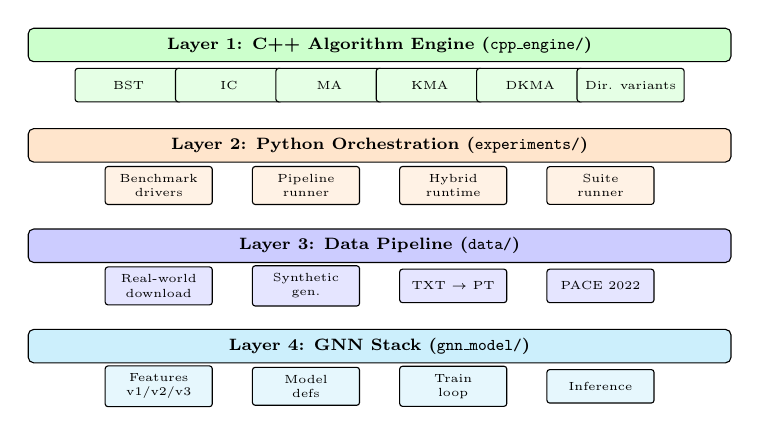
\begin{tikzpicture}[
				scale=0.85, transform shape,
				layer/.style={draw, rounded corners=2pt,
						minimum width=10.5cm, minimum height=0.5cm,
						font=\scriptsize\bfseries, align=center},
				module/.style={draw, rounded corners=1pt,
						minimum width=1.6cm, minimum height=0.5cm,
						font=\tiny, align=center},
				arr/.style={->, >=Stealth, thick, gray!70}]

			% Layer 1: C++ Engine
			\node[layer,fill=green!20] (cpp) at (0,3.0)
			{Layer 1: C++ Algorithm Engine (\texttt{cpp\_engine/})};
			\node[module,fill=green!10] (cppbst) at (-3.75,2.4) {BST};
			\node[module,fill=green!10] (cppic)  at (-2.25,2.4) {IC};
			\node[module,fill=green!10] (cppma)  at (-0.75,2.4) {MA};
			\node[module,fill=green!10] (cppkma) at (0.75,2.4) {KMA};
			\node[module,fill=green!10] (cppdkma) at (2.25,2.4) {DKMA};
			\node[module,fill=green!10] (cppdir) at (3.75,2.4) {Dir. variants};

			% Layer 2: Python Orchestration
			\node[layer,fill=orange!20] (pyorch) at (0,1.5)
			{Layer 2: Python Orchestration (\texttt{experiments/})};
			\node[module,fill=orange!10] (bench) at (-3.3,0.9) {Benchmark\\drivers};
			\node[module,fill=orange!10] (pipe)  at (-1.1,0.9) {Pipeline\\runner};
			\node[module,fill=orange!10] (hybr)  at (1.1,0.9) {Hybrid\\runtime};
			\node[module,fill=orange!10] (suite) at (3.3,0.9) {Suite\\runner};

			% Layer 3: Data
			\node[layer,fill=blue!20] (data) at (0,0.0)
			{Layer 3: Data Pipeline (\texttt{data/})};
			\node[module,fill=blue!10] (rw)   at (-3.3,-0.6) {Real-world\\download};
			\node[module,fill=blue!10] (syn)  at (-1.1,-0.6) {Synthetic\\gen.};
			\node[module,fill=blue!10] (pt)   at (1.1,-0.6) {TXT $\to$ PT};
			\node[module,fill=blue!10] (pace) at (3.3,-0.6) {PACE 2022};

			% Layer 4: GNN
			\node[layer,fill=cyan!20] (gnn) at (0,-1.5)
			{Layer 4: GNN Stack (\texttt{gnn\_model/})};
			\node[module,fill=cyan!10] (feat) at (-3.3,-2.1) {Features\\v1/v2/v3};
			\node[module,fill=cyan!10] (mod)  at (-1.1,-2.1) {Model\\defs};
			\node[module,fill=cyan!10] (trn)  at (1.1,-2.1) {Train\\loop};
			\node[module,fill=cyan!10] (inf)  at (3.3,-2.1) {Inference};

		\end{tikzpicture}
	\end{center}
\end{frame}


% ════════════════════════════════════════════════════════════════════════════
\subsection{Results \& Evaluation}
% ════════════════════════════════════════════════════════════════════════════

\begin{frame}{Evaluation Framework}
	\tiny
	\begin{columns}[T]
		\begin{column}{0.50\textwidth}
			\begin{block}{Benchmark Output Format}
				Each benchmark run produces a CSV with:
				\begin{itemize}\setlength\itemsep{1pt}
					\item File identity \& graph metadata
					\item Algorithm / family / track tags
					\item \texttt{fvs\_size}: solution size
					\item \texttt{runtime}: wall-clock seconds
					\item \texttt{valid}: acyclicity-verified boolean
					\item \texttt{status}: completed / timeout / error
				\end{itemize}
			\end{block}
			\vspace{4pt}
			\begin{block}{Benchmark Tracks}
				\textbf{exact\_track:} compared against IC/BST optimal\\
				\textbf{heuristic\_track:} compared against MA baseline\\
				\textbf{PACE 2022:} compared against official winner
			\end{block}
		\end{column}
		\begin{column}{0.46\textwidth}
			\begin{block}{Algorithm Comparison Matrix}
				\begin{tabular}{lcc}
					\toprule
					Algorithm  & Exact      & Heuristic  \\
					\midrule
					BST        & \checkmark & --         \\
					IC         & \checkmark & --         \\
					MA         & --         & \checkmark \\
					KMA        & --         & \checkmark \\
					DKMA       & --         & \checkmark \\
					GNN-KMA v1 & --         & \checkmark \\
					GNN-KMA v2 & --         & \checkmark \\
					GNN-KMA v3 & --         & \checkmark \\
					GNN-DKMA   & --         & \checkmark \\
					\bottomrule
				\end{tabular}
			\end{block}
			\vspace{4pt}
			\begin{tcolorbox}[greenbox,fontupper=\footnotesize]
				\textbf{Resume semantics:} all benchmark
				pipelines support deterministic restart -
				interrupted runs continue from last completed file.
			\end{tcolorbox}
		\end{column}
	\end{columns}
\end{frame}


\begin{frame}{Exact solution Checker}
	\begin{block}{Results}
		\begin{tabular}{lrr}
			\toprule
			Solver                   & Mean score (\%) & Instances completed Before Timeout \\
			\midrule
			undirected\_BST\_exact   & 100.0           & 9046                               \\
			undirected\_IC\_exact    & 100.0           & 9906                               \\
			undirected\_brute\_force & 100.0           & 7263                               \\
			\bottomrule
		\end{tabular}
	\end{block}

	\vspace{6pt}
	\begin{itemize}
		\item \textbf{Instance count:} Number of instances that completed before timeout.
		\item \textbf{Mean score (100\%):} For every completed instance, the solver returned an optimal solution among the instances it finished.
		\item As all three solvers report 100\%, the \textbf{brute force}, \textbf{IC}, and \textbf{BST} exact solvers produced the same optimal answers on their completed instances.
	\end{itemize}
\end{frame}










\begin{frame}{Exact success percentage by graph size}
	\centering
	\begin{columns}[T]
		\begin{column}{0.33\textwidth}
			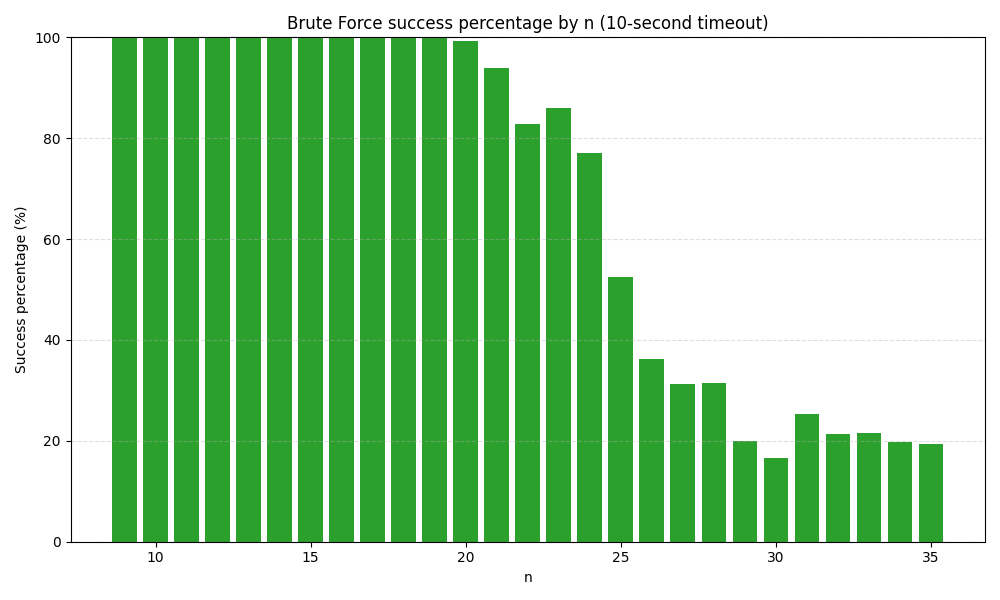
\includegraphics[width=\textwidth]{figures/brute_force_success_percentage_by_n.png}
			\vspace{3pt}
			\tiny Brute Force exact success rate vs. $n$
		\end{column}
		\begin{column}{0.33\textwidth}
			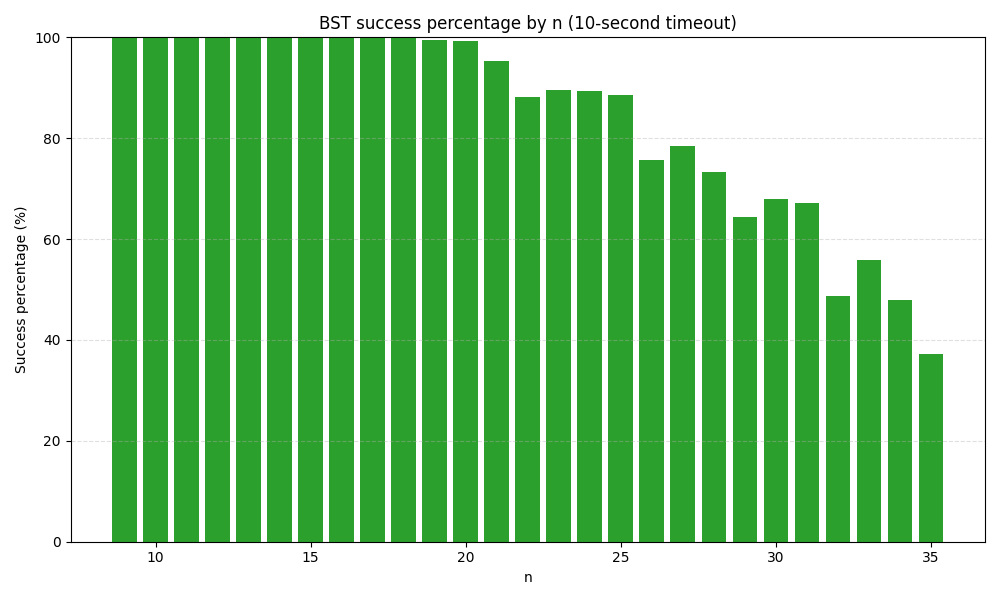
\includegraphics[width=\textwidth]{figures/BST_exact_success_percentage_by_n.png}
			\vspace{3pt}
			\tiny BST exact success rate vs. $n$
		\end{column}
		\begin{column}{0.33\textwidth}
			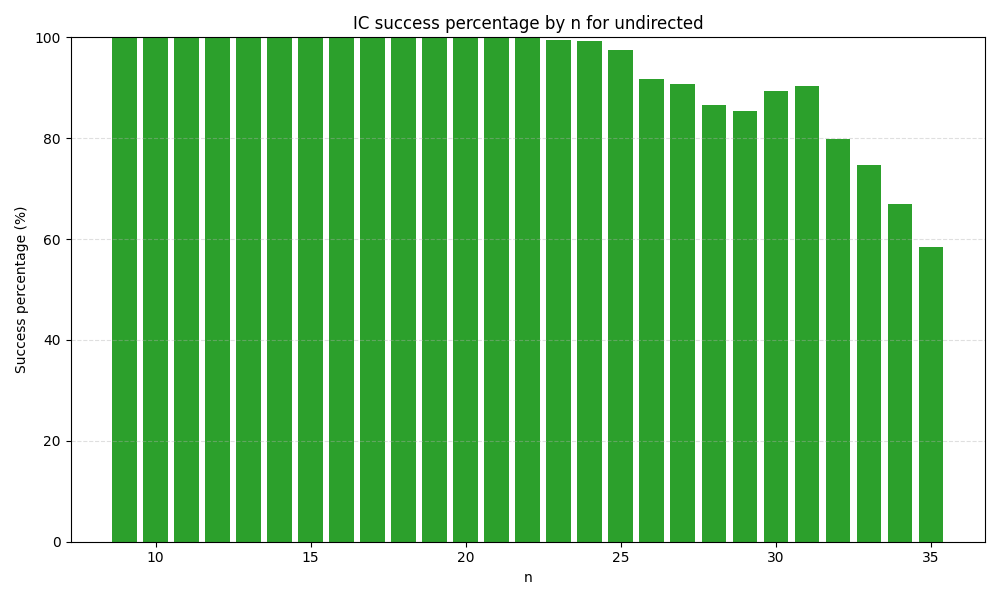
\includegraphics[width=\textwidth]{figures/undirected_ic_success_percentage_by_n.png}
			\vspace{3pt}
			\tiny IC exact success rate vs. $n$
		\end{column}
	\end{columns}
\end{frame}

\begin{frame}{Exact success percentage by solution size}
	\centering
	\begin{columns}[T]
		\begin{column}{0.49\textwidth}
			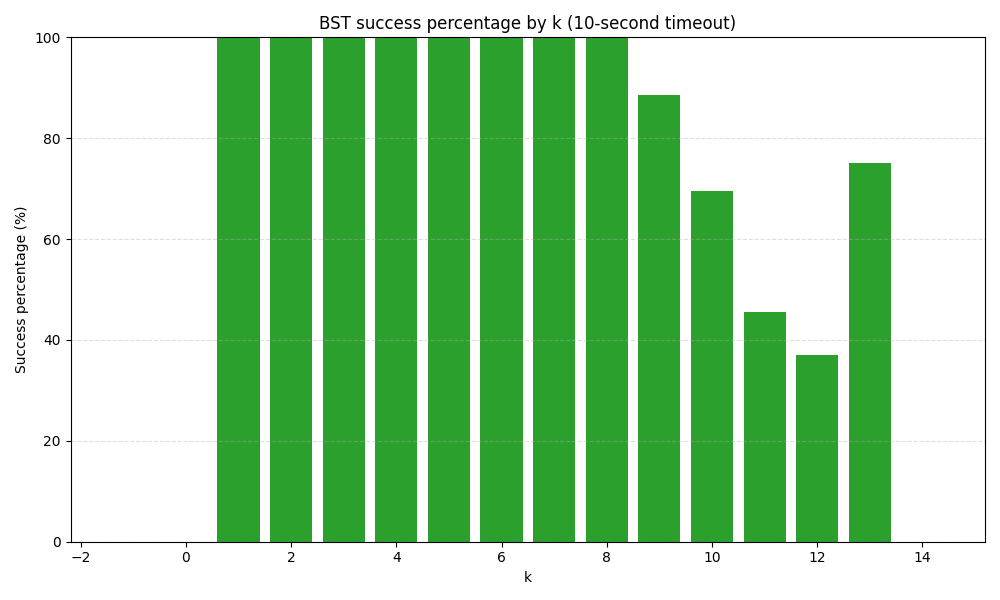
\includegraphics[width=\textwidth]{figures/BST_exact_success_percentage_by_k.png}
			\vspace{3pt}
			\tiny BST exact success rate vs. $k$
		\end{column}
		\begin{column}{0.49\textwidth}
			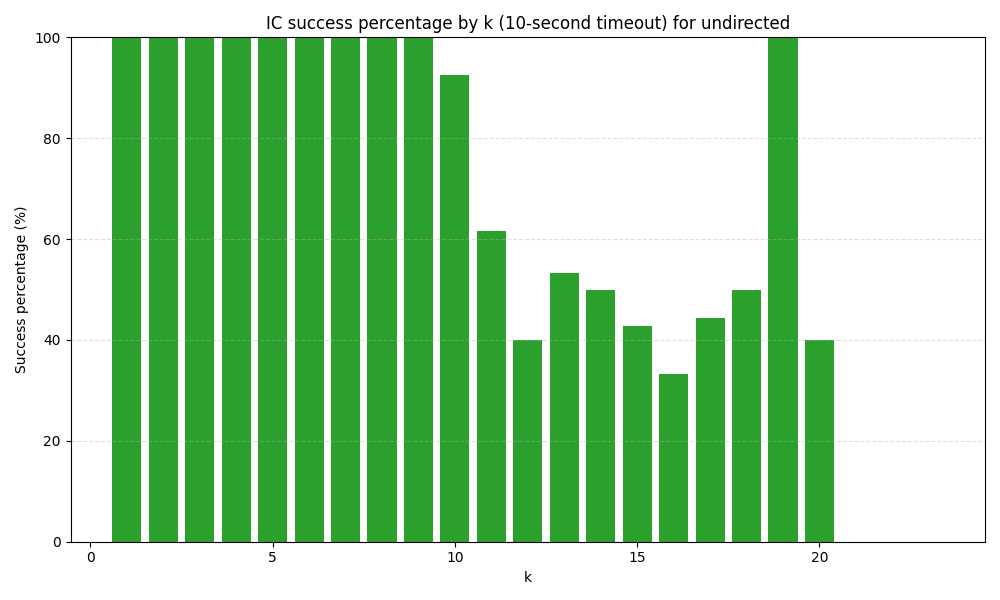
\includegraphics[width=\textwidth]{figures/undirected_ic_success_percentage_by_k.png}
			\vspace{3pt}
			\tiny IC exact success rate vs. $k$
		\end{column}
	\end{columns}
\end{frame}

\begin{frame}{Undirected runtime vs. $k$ for $n = 28$}
	\centering
	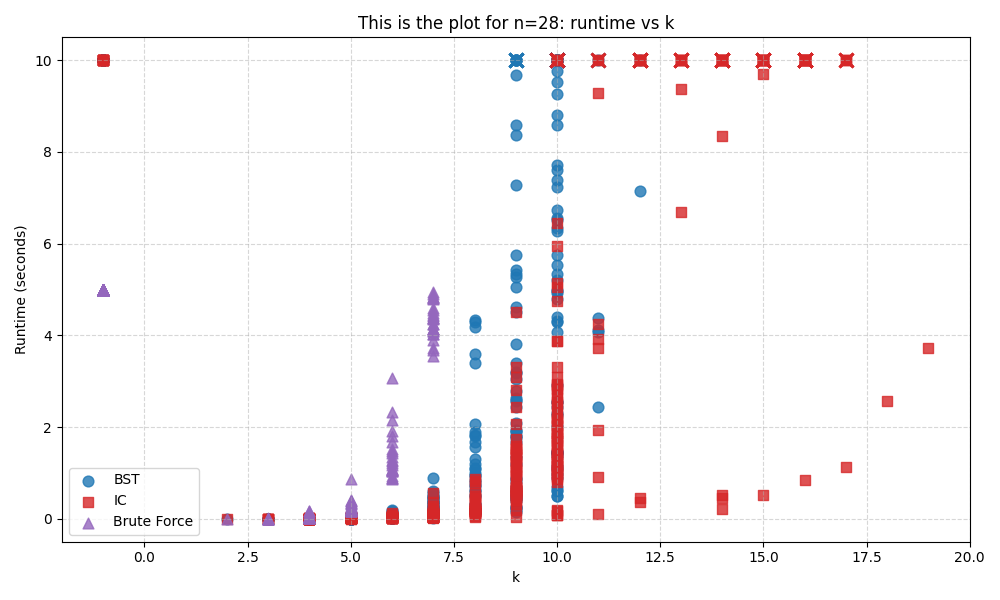
\includegraphics[width=0.88\textwidth]{figures/undirected_runtime_vs_k_for_n_28.png}
\end{frame}

\begin{frame}{Undirected runtime vs. $n$ for $k = 4$}
	\centering
	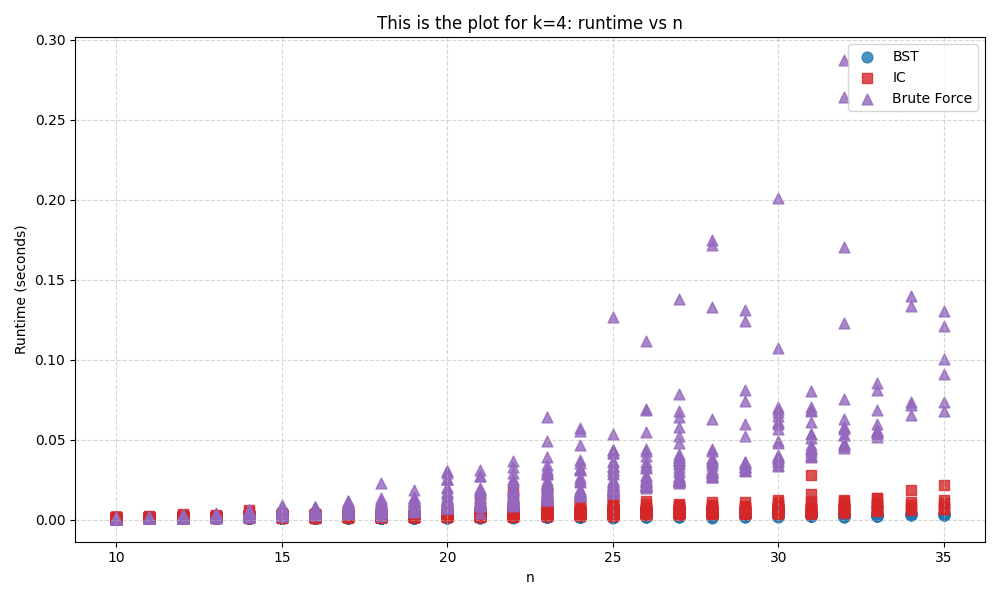
\includegraphics[width=0.88\textwidth]{figures/undirected_runtime_vs_n_for_k_4.png}
\end{frame}

\begin{frame}{Pareto analysis of solver performance}
	\centering
	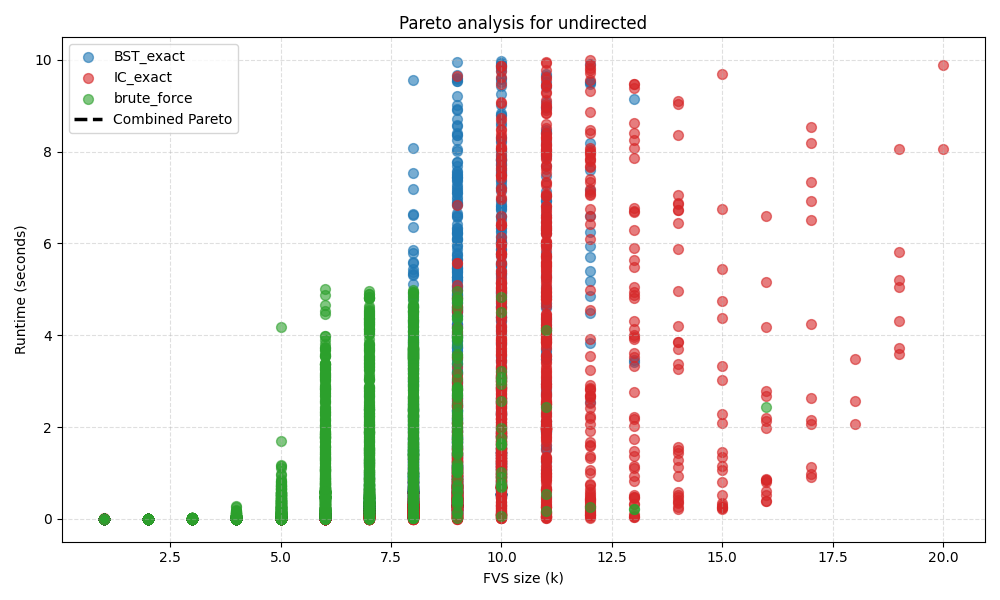
\includegraphics[width=0.88\textwidth]{figures/pareto_analysis.png}
\end{frame}

\begin{frame}{PACE 2022 test scoring}
	\begin{itemize}
		\item Each PACE 2022 problem uses a separate 100-point score for each test case.
		\item If three valid solutions $a, b, c$ have sizes 89, 91, 85 then
			$a$'s score is $100 \times \frac{85}{89}$ for that case.
		\item The score formula is $100 \times \frac{\text{OPT FVS}}{\text{solved FVS}}$.
		\item Total marks are the mean over all test case scores.
		\item For invalid FVS outputs, we use the fallback size $n$ and score accordingly.
	\end{itemize}
\end{frame}

\begin{frame}{PACE 2022 competitor benchmark}
	\begin{itemize}
		\item We benchmarked against the PACE 2022 winner implementation by Sylwester Swat.
		\item Author: Sylwester Swat, Pozna\'n University Of Technology.
		\item GitHub: \url{https://github.com/swacisko/pace-2022}
		\item His reported score: \textbf{99.9117834156}.
		\item We ran all available heuristics on the PACE 2022 test cases and kept this result as our competitor baseline.
		\item Because the winner's score is so close to 100, this gives us a realistic reference for actual PACE scoring.
	\end{itemize}
\end{frame}

\begin{frame}{PACE 2022 heuristic results (descending score)}
	\small
	\begin{itemize}
		\item \textbf{pace2022 winner}: 100.0000 (based on 200 instances) - total time=600.00s
		\item \textbf{directed KMA heuristic 90}: 78.9312 (based on 200 instances) - total time=18709.90s
		\item \textbf{directed GNN-KMA-3 0.85 heuristic 30}: 78.6449 (based on 200 instances) - total time=15617.54s
		\item \textbf{directed GNN-KMA-3 0.95 heuristic 30}: 77.7510 (based on 200 instances) - total time=15302.61s
		\item \textbf{directed GNN-KMA heuristic 30}: 76.9814 (based on 200 instances) - total time=8380.73s
		\item \textbf{directed DKMA heuristic 30}: 76.4942 (based on 200 instances) - total time=8367.24s
		\item \textbf{directed KMA heuristic 30}: 76.3657 (based on 200 instances) - total time=7820.26s
		\item \textbf{directed GNN-KMA-3 small 0.9 heuristic 30}: 76.2655 (based on 200 instances) - total time=16480.64s
		\item \textbf{directed DKMA heuristic 15}: 75.8974 (based on 200 instances) - total time=4641.90s
		\item \textbf{directed KMA heuristic 15}: 75.6944 (based on 200 instances) - total time=4209.18s
		\item \textbf{directed MA heuristic 90}: 71.8443 (based on 200 instances) - total time=18281.50s
		\item \textbf{directed MA heuristic 60}: 70.6738 (based on 200 instances) - total time=12483.29s
		\item \textbf{directed MA heuristic 30}: 68.6420 (based on 200 instances) - total time=6565.01s
	\end{itemize}
\end{frame}

\begin{frame}{All solvers mean score}
	\centering
	
\includegraphics[width=0.60\textwidth]{figures/all_solvers_mean_score.png}
\end{frame}

\begin{frame}{MA models mean score}
	\centering
	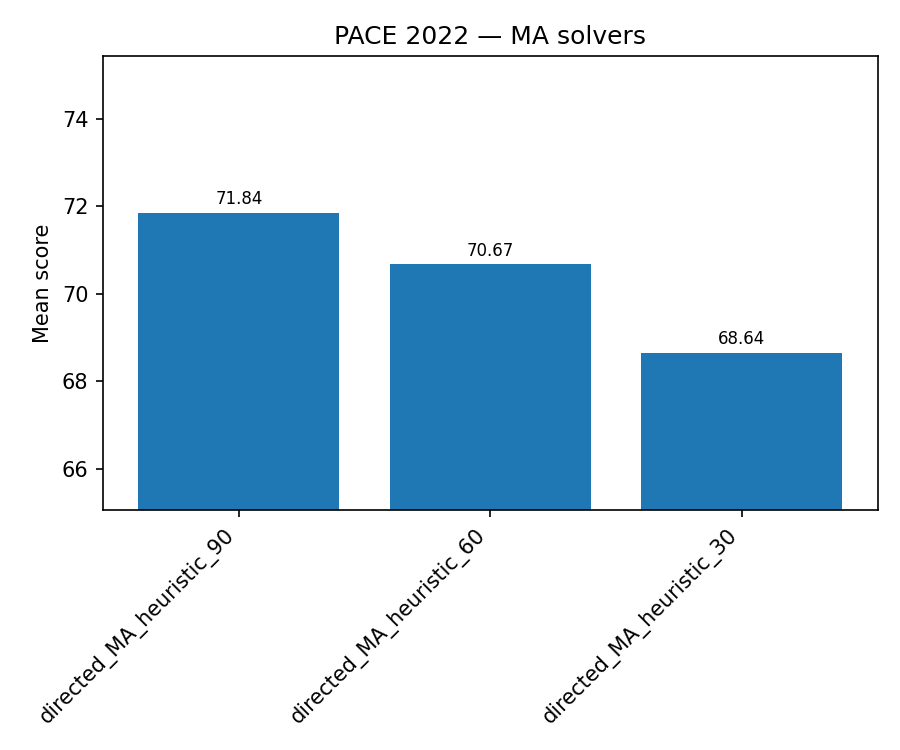
\includegraphics[width=0.55\textwidth]{figures/models_MA_mean_score.png}
\end{frame}

\begin{frame}{KMA models mean score}
	\centering
	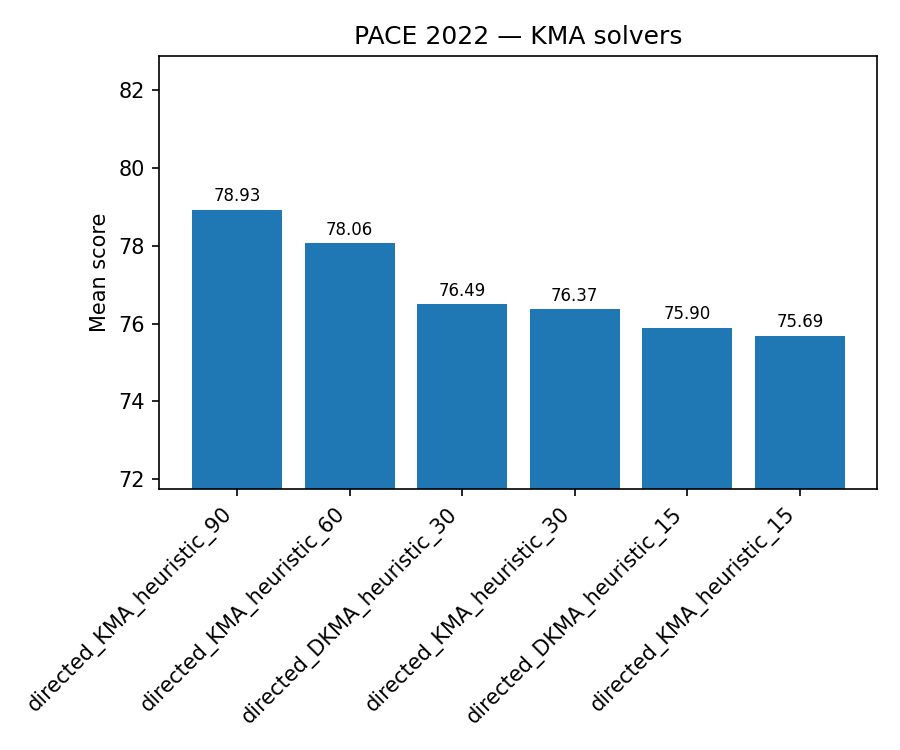
\includegraphics[width=0.55\textwidth]{figures/models_KMA_mean_score.png}
\end{frame}

\begin{frame}{DKMA models mean score}
	\centering
	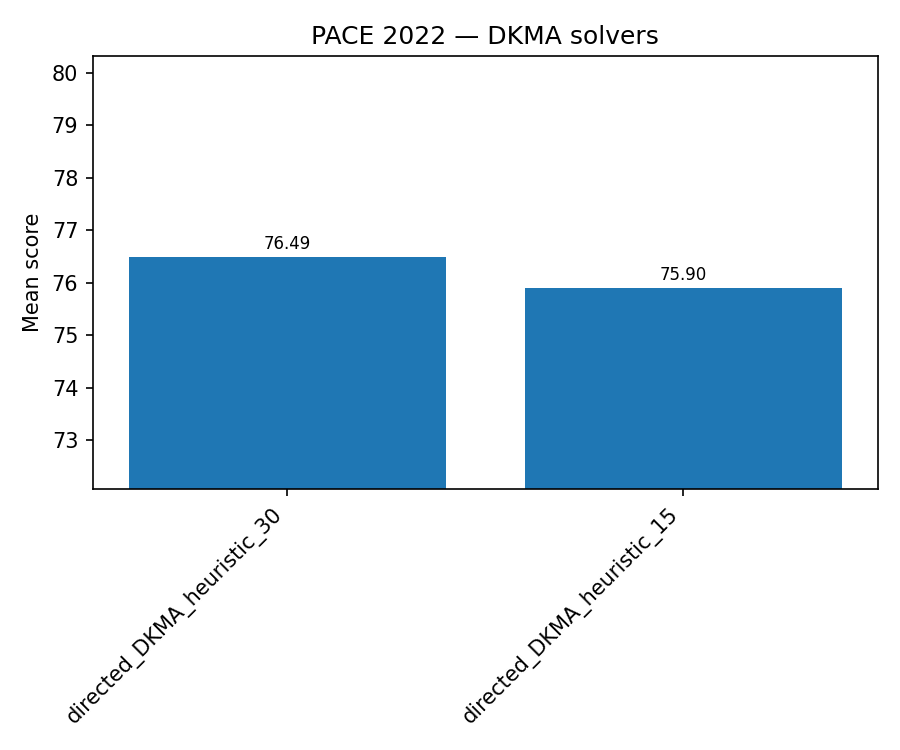
\includegraphics[width=0.55\textwidth]{figures/models_DKMA_mean_score.png}
\end{frame}

\begin{frame}{Group 15 mean score}
	\centering
	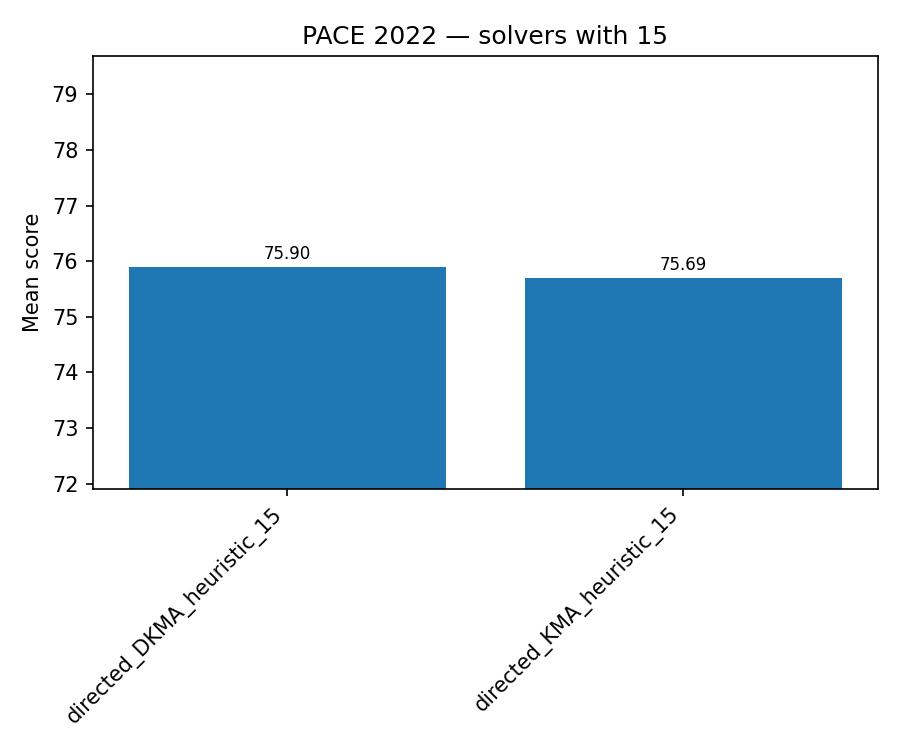
\includegraphics[width=0.55\textwidth]{figures/group_15_mean_score.png}
\end{frame}

\begin{frame}{Group 30 mean score}
	\centering
	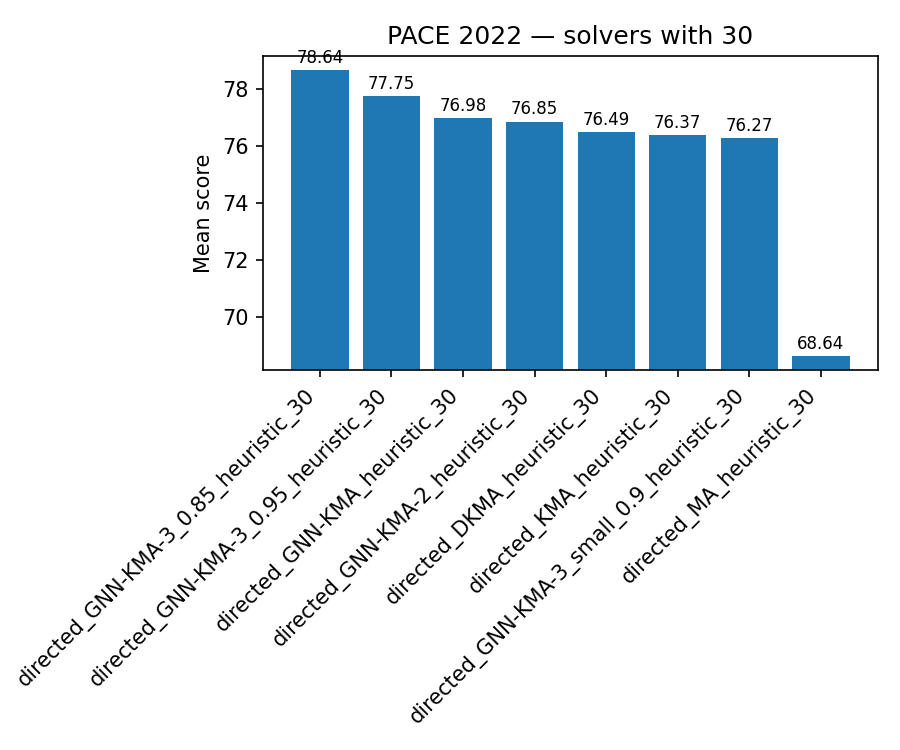
\includegraphics[width=0.55\textwidth]{figures/group_30_mean_score.png}
\end{frame}

\begin{frame}{Group 60 mean score}
	\centering
	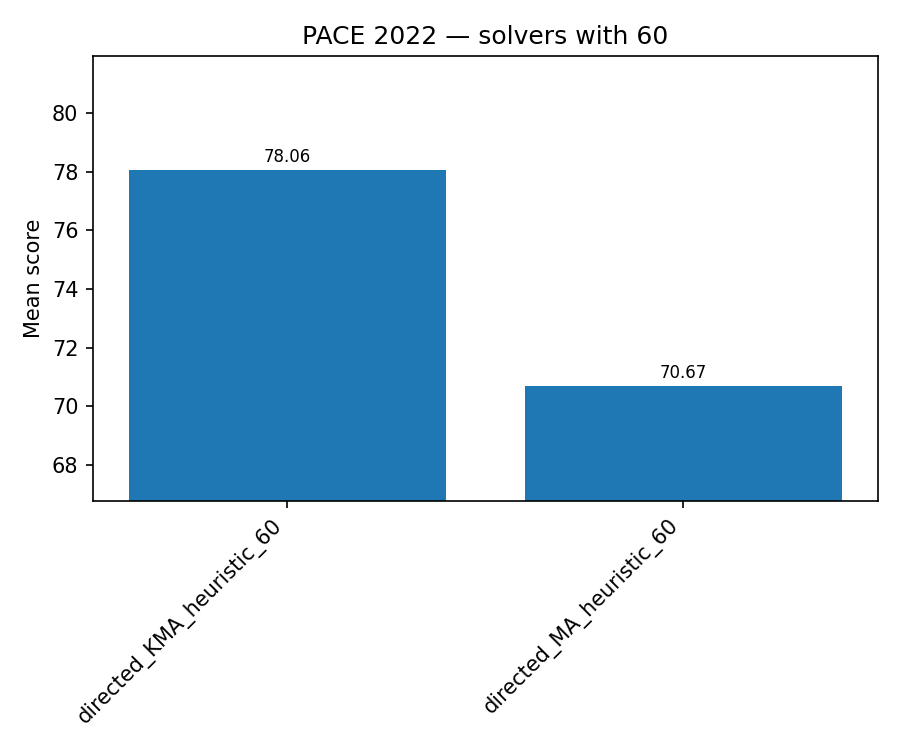
\includegraphics[width=0.55\textwidth]{figures/group_60_mean_score.png}
\end{frame}

\begin{frame}{Group 90 mean score}
	\centering
	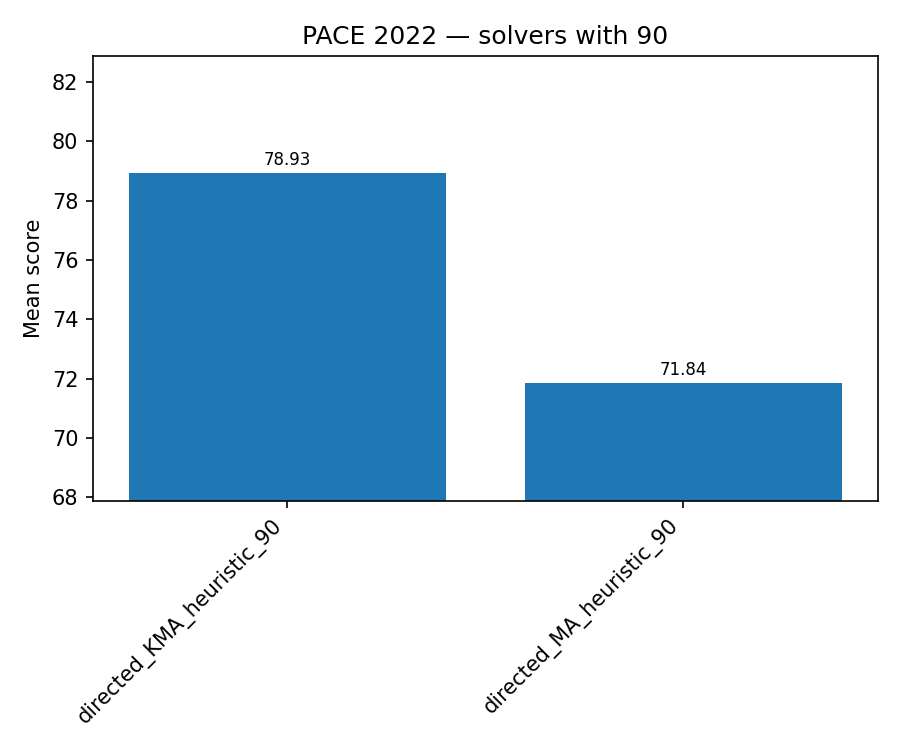
\includegraphics[width=0.55\textwidth]{figures/group_90_mean_score.png}
\end{frame}

\begin{frame}{GNN models mean score}
	\centering
	
\includegraphics[width=0.55\textwidth]{figures/models_GNN_mean_score.png}
\end{frame}

% ════════════════════════════════════════════════════════════════════════════
\section{Conclusions}
% ════════════════════════════════════════════════════════════════════════════

\begin{frame}{Summary \& Contributions}
	\tiny
	\begin{columns}[T]
		\begin{column}{0.47\textwidth}
			\begin{block}{\faCode~Algorithm Contributions}
				\begin{itemize}\setlength\itemsep{2pt}
					\item \highlight{KMA}: first-class kernelization (SCC reduction
					      for directed; degree-2 bypass for undirected) integrated
					      with C++ memetic search
					\item \highlight{DKMA}: dynamic re-kernelization loop,
					      SHORTONE contractions \cite{langedal2022},
					      topological diversification,
					      gain local search (1-1 / 2-1 swaps)
					\item \highlight{GNN-KMA v1/v2/v3}: progressive feature and
					      architecture improvements (GraphSAGE → GATv2 \cite{brody2022},
					      3 → 16 channels, NLL → asymmetric precision loss)
					\item \highlight{GNN-DKMA}: GNN guidance + dynamic kernelization
				\end{itemize}
			\end{block}
		\end{column}
		\begin{column}{0.47\textwidth}
			\begin{block}{\faDatabase~Dataset Contributions}
				\begin{itemize}\setlength\itemsep{2pt}
					\item 100K undirected + 100K directed labelled FVS instances
					\item 5 graph families, 2 difficulty tracks, real+synthetic mix
					\item Solver-verified ground-truth labels (IC for exact,
					      KMA for heuristic)
					\item Publicly released on Kaggle (100K and 20K versions)
					\item PACE 2022 integration for real-world benchmarking
				\end{itemize}
			\end{block}
			\vspace{4pt}
			\begin{tcolorbox}[greenbox,fontupper=\footnotesize]
				\faGithub~\textbf{GitHub:}\\
				{\tiny\url{https://github.com/TAR2003/Feedback_Vertex_Set_Problem_Algorithm_Project_4-2}}\\[4pt]
				\faDatabase~\textbf{Dataset (100K):}\\
				{\tiny\url{https://www.kaggle.com/datasets/tawkirazizrahman/fvs-synthetic-dataset-100k}}\\[2pt]
				\faDatabase~\textbf{Dataset (20K):}\\
				{\tiny\url{https://www.kaggle.com/datasets/tawkirazizrahman/fvs-synthetic-dataset-20k}}
			\end{tcolorbox}
		\end{column}
	\end{columns}
\end{frame}

% ════════════════════════════════════════════════════════════════════════════
%  REFERENCES
% ════════════════════════════════════════════════════════════════════════════
\begin{frame}[allowframebreaks]{References}
	\begin{thebibliography}{99}
		\scriptsize
		\bibitem{karp1972}
		R.M.~Karp,
		``Reducibility among combinatorial problems,''
		in \emph{Complexity of Computer Computations}, 1972, pp.~85--103.

		\bibitem{becker2000}
		A.~Becker and D.~Geiger,
		``Optimization of Pearl's method of conditioning and greedy-like approximation
		algorithms for the weighted maximum acyclic subgraph problem,''
		\emph{Artificial Intelligence}, vol.~105, pp.~1--2, 1996.

		\bibitem{thomasse2010}
		S.~Thomassé,
		``A $4k^2$ kernel for feedback vertex set,''
		\emph{ACM Trans.\ Algorithms}, vol.~6, no.~2, 2010.

		\bibitem{reed2004}
		B.~Reed, K.~Smith, and A.~Vetta,
		``Finding odd cycle transversals,''
		\emph{Operations Research Letters}, vol.~32, no.~4, 2004.

		\bibitem{cygan2015}
		M.~Cygan \emph{et al.},
		\emph{Parameterized Algorithms}.
		Springer, 2015.

		\bibitem{chen2008dfvs}
		J.~Chen, Y.~Liu, S.~Lu, B.~O'Sullivan, and I.~Razgon,
		``A fixed-parameter algorithm for the directed feedback vertex set problem,''
		\emph{J.~ACM}, vol.~55, no.~5, 2008.

		\bibitem{lust2010}
		T.~Lust and J.~Teghem,
		``The multiobjective multidimensional knapsack problem: a survey and a new approach,''
		\emph{Int.\ Trans.\ Oper.\ Res.}, 2010.
			{\footnotesize(Memetic algorithm framework reference.)}

		\bibitem{pace2022}
		G.~Grossmann, M.~Heuer, P.~Schulz, and D.~Strash,
		``Targeted solution methods for the minimum feedback vertex set problem,''
		in \emph{Proc.\ 17th IPEC}, LIPIcs vol.~249, 2022,
		doi:10.4230/LIPIcs.IPEC.2022.26.

		\bibitem{esa2022}
		A.~Figiel, V.~Froese, A.~Nichterlein, and R.~Niedermeier,
		``Improved parameterized algorithms for the directed feedback vertex set problem,''
		in \emph{Proc.\ ESA 2022}, LIPIcs, 2022,
		doi:10.4230/LIPIcs.ESA.2022.53.

		\bibitem{langedal2022}
		K.~Langedal, J.~Langguth, F.~Manne, and D.~Strash,
		``Efficient minimum weight vertex cover heuristics using graph neural networks'' (Mount-Doom FVS solver),
		Zenodo, 2022, doi:10.5281/zenodo.6630611.

		\bibitem{hamilton2017}
		W.~Hamilton, Z.~Ying, and J.~Leskovec,
		``Inductive representation learning on large graphs'' (GraphSAGE),
		in \emph{NeurIPS}, 2017.

		\bibitem{brody2022}
		S.~Brody, U.~Alon, and E.~Yahav,
		``How attentive are graph attention networks?'' (GATv2),
		in \emph{ICLR}, 2022.

		\bibitem{dwivedi2021}
		V.P.~Dwivedi \emph{et al.},
		``Benchmarking graph neural networks,''
		\emph{JMLR}, vol.~24, no.~43, 2023.
			{\footnotesize(RWSE/positional encoding reference.)}

		\bibitem{ahmed2015}
		N.K.~Ahmed, J.~Neville, R.A.~Rossi, and N.~Duffield,
		``Efficient graphlet counting for large networks,''
		in \emph{ICDM}, 2015.

		\bibitem{batagelj2003}
		V.~Batagelj and M.~Zaversnik,
		``An $O(m)$ algorithm for cores decomposition of networks,''
		\emph{arXiv:cs/0310049}, 2003.

		\bibitem{tarjan1972}
		R.E.~Tarjan,
		``Depth-first search and linear graph algorithms,''
		\emph{SIAM J.~Comput.}, vol.~1, no.~2, 1972.

		\bibitem{barabasi1999}
		A.-L.~Barabási and R.~Albert,
		``Emergence of scaling in random networks,''
		\emph{Science}, vol.~286, 1999.

		\bibitem{watts1998}
		D.J.~Watts and S.H.~Strogatz,
		``Collective dynamics of `small-world' networks,''
		\emph{Nature}, vol.~393, 1998.

		\bibitem{erdos1959}
		P.~Erdős and A.~Rényi,
		``On random graphs I,''
		\emph{Publicationes Mathematicae}, vol.~6, 1959.
	\end{thebibliography}
\end{frame}

% ─── Final slide ──────────────────────────────────────────────────────────────
\begin{frame}[plain]
	\begin{tikzpicture}[remember picture, overlay]
		\fill[darkblue] (current page.south west) rectangle (current page.north east);
	\end{tikzpicture}
	\begin{center}
		\vspace{1.8cm}
		{\color{white}\Huge\bfseries Thank You}\\[14pt]
		{\color{accentblue!80!white}\large Questions \& Discussion}\\[28pt]

		\begin{tabular}{ll}
			\color{white}\faGithub   & \color{white}{\small\url{https://github.com/TAR2003/Feedback_Vertex_Set_Problem_Algorithm_Project_4-2}} \\[6pt]
			\color{white}\faDatabase & \color{white}{\small\url{https://www.kaggle.com/datasets/tawkirazizrahman/fvs-synthetic-dataset-100k}}  \\[6pt]
			\color{white}\faDatabase & \color{white}{\small\url{https://www.kaggle.com/datasets/tawkirazizrahman/fvs-synthetic-dataset-20k}}   \\
		\end{tabular}
	\end{center}
\end{frame}

\end{document}

